\documentclass[a4paper]{report}
\input{../preamble.tex}
\title{Description Logic}

% account for different counting scheme in lecture
\counterwithout*{definition}{section}
\counterwithin*{definition}{chapter}
\renewcommand{\thedefinition}{\arabic{chapter}.\arabic{definition}}

% ensure right spacing around squared operators and relations
\let\helpercap\sqcap
\renewcommand{\sqcap}{\mathbin{\helpercap}}
\let\helpercup\sqcup
\renewcommand{\sqcup}{\mathbin{\helpercup}}
\let\helpersSub\sqsubseteq
\renewcommand{\sqsubseteq}{\mathrel{\helpersSub}}
\DeclareMathSymbol{:}{\mathop}{operators}{"3A}

\begin{document}
	\selectlanguage{english}
	\maketitle
	\tableofcontents
	%% start of lectures
	% Chapter counting starts at 0
\setcounter{chapter}{-1}
\chapter{Introduction}
This is my transcript of the lecture "Description Logic" held by Prof. Dr. Franz Baader at TU Dresden in the summer semester 2021.
The lecture is based on the book "An Introduction to Description Logic" \cite{baader_dl_17} co-authored by Prof. Baader.

\chapter{Introduction}
\lecture{1}{18.04.2021}{}
Description Logic (DL) is a subfield of knowledge representation which intern is a subfield of Artificial Intelligence.
Note, that there is not \textbf{one} DL, but many different ones, most of which can be seen as fragments of FOL.
The general goal of Knowledge Representation and therefor of DL can be summarized as follows:
\begin{itemize}
	\item formalism: well-defined syntax and unambiguous semantics
	\item high-level description: only relevant aspects need to be represented
	\item intelligent applications: ability to infer implicit knowledge from the explicitly represented one
	\item effective: practical for reasoning tools and efficient implementable
\end{itemize}
Especially the latter point is interesting, since FOL is undecidable.
Therefore we must strike the right balance when it comes to expressive power.
Too low and not all the relevant knowledge can be presented, too high and reasoning becomes inefficient (or impossible).

The reasoning procedures used for processing the knowledge represented by a DL should satisfy the following properties:
\begin{itemize}
	\item soundness: Positive answers are indeed correct. 
	\item correctness: All positive answers are found, e.g.\ negative answers are correct.
	\item termination: There will always be an answer in finite time.
\end{itemize}
The procedure should furthermore be as efficient and as practical as possible.

To automatically reason about implicitly represented knowledge in a DL, one has to formalize the following:
\begin{itemize}
	\item syntax and semantics used in the DL (\textbf{description language}),
	\item the terminological knowledge of the application domain (\textbf{TBox}),
	\item the facts known about the specific "world" instance (\textbf{ABox}).
\end{itemize}

\chapter{A basic Description Logic}
In this chapter we will have a look at a basic DL called $\mathcal{ALC}$. 
The names of DLs follow a common naming scheme:
\begin{itemize}
	\item the basic language is called "attributive language"
	\item additional constructors are abbreviated with letters that are added after $ \mathcal{AL} $ 
	\item $ \mathcal{C} $ stands for \textit{complement}, i.e., $ \mathcal{ALC} $ is obtained from $ \mathcal{AL} $ by adding the complement ($ \neg $) operator
\end{itemize}

\section{The description language of $\mathcal{ALC}$}
\subsection{Syntax and semantics of $\mathcal{ALC}$}
\begin{definition}[Syntax of $\mathcal{ALC}$]
	Let $\mathscr{C}$ and $\mathscr{R}$ be disjoint sets of concept names and role names, respectively.
	$\mathcal{ALC}$-concept descriptions are inductively defined.
	\begin{itemize}
		\item If $ A \in \mathscr{C} $, then $ A $ is an $ \mathcal{ALC}$-concept description.
		\item If $ C,D $ are $ \mathcal{ALC}$-concept description, and $ r \in \mathscr{R} $, then the following are $\mathcal{ALC}$-concept descriptions:
			\begin{itemize}
				\item $ C \sqcap D $ (conjunction)
				\item $ C \sqcup D $ (disjunction)
				\item $ \neg C $ (negation)
				\item $ \forall r.C $ (value restriction)
				\item $ \exists r.C $ (existential restriction)
			\end{itemize}
	\end{itemize}
\end{definition}

\begin{note}
	One could equivalently define $\bot$ and $\top$ as concept descriptions.
	The main differences lie in the structure of induction proves and the length of formulas, that may be used in complexity analysis.
\end{note}

\begin{notation}
	We allow ourselves the use of parentheses for better structure and to define the following abbreviations:
	\begin{itemize}
		\item $ \top \coloneqq A \sqcup \neg A $ (top)
		\item $ \bot \coloneqq A \sqcap \neg A $ (bottom)
		\item $ C \Rightarrow D \coloneqq \neg C \sqcup D $ (implication)
	\end{itemize}
	Furthermore, we will use these conventions:
	\begin{itemize}
		\item Concept names are called \textit{atomic}.
		\item All other $\mathcal{ALC}$-concept descriptions are called \textit{complex}.
		\item We often abbreviate \textit{$\mathcal{ALC}$-concept description} with \textit{concept description} or just \textit{concept}.
		\item We often use $A, B$ for concept names, $C, D$ for (possibly) complex concepts and $r, s$ for role names.
		\item When talking about concrete elements of $\mathscr{C}$ or $\mathscr{R}$ we will use capitalized concept names and lowercased role names.
	\end{itemize}
\end{notation}

\begin{example}
	Here are some examples of the $\mathcal{ALC}$-syntax.
	Although the naming is chosen to have intuitive meaning, we have not defined a formal semantics of this description language yet.
	\begin{itemize}
		\item $ \var{Person} \sqcap \var{Female}$
		\item $ \var{Student} \sqcap \forall \var{attends}.(\var{Lecture}\sqcap \neg \var{Boring})$
	\end{itemize}
\end{example}

	\input{lec2.tex}
	\lecture{3}{20.04.2021}{}
\begin{example}
	Here is an example of an acyclic TBox:
	\begin{itemize}
		\item $ \var{Woman} \equiv \var{Person} \sqcap \var{Female}$
		\item $\var{Man} \equiv \var{Person} \sqcap \neg \var{Female}$
	\end{itemize}
	$\left\{ \var{Woman}, \var{Man} \right\} $ are the defined concepts and $\left\{ \var{Person}, \var{Female} \right\}$ are primitive concepts.
\end{example}

\begin{prop}
	For every acyclic TBox $\mathcal{T}$ we can effectively construct an equivalent acyclic TBox $ \widehat{\mathcal{T}}$
	such that the right-hand sides of concept definitions in $\widehat{\mathcal{T}}$ contain only primitive concepts.
\end{prop}
\begin{proof}
	By recursively expanding the (finitely many and acyclic) definitions.
\end{proof}

Given an acyclic TBox $\mathcal{T}$, a primitive interpretation $\mathcal{J}$ for $\mathcal{T}$ 
consists of a nonempty set $\Delta^{\mathcal{J}}$ together with an extension mapping $\cdot^{\mathcal{J}}$, that maps
\begin{itemize}
	\item primitive concepts $P$ to sets $P^{\mathcal{J}} \subseteq \Delta^{\mathcal{J}}$ 
	\item role names r to binary relations $r^\mathcal{J} \subseteq \Delta^{\mathcal{J}} \times \Delta^{\mathcal{J}}$
\end{itemize}
The interpretation $\mathcal{I}$ is an extension of the primitive interpretation $\mathcal{J}$ iff $\Delta^{\mathcal{J}} = \Delta^{\mathcal{I}}$ and
 \begin{itemize}
	\item $P^{\mathcal{J}} = P^{\mathcal{I}}$ for all primitive concepts $P$ 
	\item $r^{\mathcal{J}} = r^{\mathcal{I}}$ for all role names $r$
\end{itemize}

\begin{corollary}
	Let $\mathcal{T}$ be an acyclic TBox.
	Any primitive interpretation $\mathcal{J}$ for $\mathcal{T}$ has a unique extension to a model of $\mathcal{T}$.
\end{corollary}
\begin{proof}
	First construct the expanded TBox $\widehat{\mathcal{T}}$ for $\mathcal{T}$.
	Obviously, $\mathcal{T}$ and $\widehat{\mathcal{T}}$ have the same primitive and defined concepts.
	Let $\mathcal{J}$ be a primitive interpretation.
	We define its extension $\mathcal{I}$ as follows:
	For every defined concept $A$, let $A \equiv \hat{C}$ be its definition in $\widehat{\mathcal{T}}$.
	Since $\hat{C}$ contains only primitive concepts, $\hat{C}^{\mathcal{J}}$ is well-defined and we set $A^{\mathcal{I}} \coloneqq \hat{C}^{\mathcal{J}}$
	\begin{enumerate}
		\item $\mathcal{I}$ is a model of $\mathcal{T}$ : \newline
			By definition it is a model of $\widehat{\mathcal{T}}$ and we know $\mathcal{T}$ and $\widehat{\mathcal{T}}$ are equivalent.
		\item $\mathcal{I}$ is unique: \newline
			Assume that $\mathcal{I}'$ is another model of $\mathcal{T}$ that extends $\mathcal{J}$.
			Then $\mathcal{I}'$ is also a model of $\widehat{\mathcal{T}}$, and thus the following holds for all defined concepts $A$,
			where $A \equiv \hat{C}$ is the definition of $A$ in $\widehat{\mathcal{T}}$ :
			\[
				A^{\mathcal{I}'} = \hat{C}^{\mathcal{I}'} = \hat{C}^{\mathcal{J}} = \hat{C}^{\mathcal{I}} = A^{\mathcal{I}}
			. \qedhere \]
	\end{enumerate}
\end{proof}

\subsection*{Relationship with FOL}
$\mathcal{ALC}$-TBoxes can be translated into FOL:
\[
	\tau(\mathcal{T}) \coloneqq \bigwedge_{C \sqsubseteq D \in \mathcal{T}} \forall x.\left( \tau_x(C) \rightarrow \tau_x(D) \right)
.\]

\begin{lemma}
	Let $\mathcal{T}$ be a TBox, then $\mathcal{T}$ and $\tau(\mathcal{T})$ have the same models.
\end{lemma}
\begin{proof}
	trivial.
\end{proof}

\newpage
\section{Assertional knowledge}
\subsection{$\mathcal{ALC}$ ABoxes}
While concepts make statements about sets of individuals, we now want to state knowledge about specific individuals.

\begin{definition}[Assertions and ABoxes]
	An assertion is of the form $a:C$ (concept assertion) or $(a,b):r$ (role assertion),
	where $C$ is a concept description, $r$ is a role and $a,b$ are individual names from a set $\mathscr{I}$ of such names (disjoint with $\mathscr{C} \uplus \mathscr{R}$).
	An ABox is a finite set of assertions.
	An Interpretation $\mathcal{I}$ is a model of an ABox $\mathcal{A}$ if it satisfies all its assertions:
	\begin{itemize}
		\item $a^{\mathcal{I}} \in C^{\mathcal{I}}$ for all $a:C \in \mathcal{A}$ 
		\item $(a^{\mathcal{I}}, b^{\mathcal{I}}) \in r^{\mathcal{I}}$ for all $(a,b):r \in \mathcal{A}$
	\end{itemize}
\end{definition}

\begin{example}
	An example of an ABox:
	\begin{itemize}
		\item $ \var{MAX}: \var{Student}$
		\item $(\var{MAX}, \var{DL}): \var{interested}$
	\end{itemize}
\end{example}

\subsection{Relationship with FOL}
$\mathcal{ALC}$-ABoxes can be translated into FOL:
\[
	\tau(\mathcal{A}) \coloneqq \bigwedge_{a:C \in \mathcal{A}} \tau_{x}(C)(a) \land \bigwedge_{(a,b):r \in \mathcal{A}} r(a,b)
.\]

\begin{lemma}
	Let $\mathcal{A}$ be an ABox and $\tau(\mathcal{A})$ its translation into FOL.
	Then $\mathcal{A}$ and $\tau (\mathcal{A})$ have the same models.
\end{lemma}
\begin{proof}
	trivial.
\end{proof}

\newpage
\section{Knowledge Bases}
We will now combine the TBox and the ABox to form the foundation for reasoning in an DL.
\begin{definition}
	A knowledge base $\mathcal{K} = (\mathcal{T}, \mathcal{A})$ consists of a TBox $\mathcal{T}$ and an ABox $\mathcal{A}$.
	The interpretation $\mathcal{I}$ is a model of the knowledge base $\mathcal{K}$, iff it is a model of its TBox and its ABox.
\end{definition}
The FOL-translation of a knowledge base is easy, given its components:
\[
\tau(\mathcal{K}) \coloneqq \tau(\mathcal{T}) \land \tau(\mathcal{A})
.\] 
\begin{lemma}
	Let $\mathcal{K}$ be a knowledge base and $\tau(\mathcal{K})$ its translation into FOL.
	Then $\mathcal{K}$ and $\tau(\mathcal{K})$ have the same models.
\end{lemma}

\subsection{Additional constructors}
Individual names can also be used as concept constructors.
\begin{definition*}[$\mathcal{O}$ in the naming scheme.]
	This allows \textbf{nominals} $\left\{ a \right\} $ for $a \in \mathscr{I}$ with the semantics
	\[
	\left\{ a \right\} ^{\mathcal{I}} \coloneqq \left\{ a^{\mathcal{I}} \right\} 
	.\] 
	In this case, the ABox can be expressed using GCIs:
	\begin{itemize}
		\item $a:C$ is expressed as $\left\{ a \right\} \sqsubseteq C$
		\item $(a,b):r$ is expressed as $\left\{ a \right\} \sqsubseteq \exists r.\left\{ b \right\} $
	\end{itemize}
\end{definition*}

\newpage
\section{Reasoning Problems and Services}
\begin{definition}[terminological reasoning]
	Let $\mathcal{T}$ be a TBox and $C,D$ be (possibly) complex concept descriptions.
	We then consider the following decision problems:
	\begin{enumerate}
		\item Satisfiability: $C$ is satisfiable w.r.t.\ $\mathcal{T}$ iff
			$C^{\mathcal{I}} \neq \emptyset$ for some model $\mathcal{I}$ of $\mathcal{T}$.
		\item Subsumption: $C$ is subsumed by $D$ w.r.t.\ $\mathcal{T}$ $\left( C \sqsubseteq_{\mathcal{T}} D \right)$ iff
			$C^{\mathcal{I}} \subseteq D^{\mathcal{I}}$ for all models $\mathcal{I}$ of $\mathcal{T}$.
		\item Equivalence: $C$ is equivalent to $D$ w.r.t.\ $\mathcal{T}$ $\left( C \equiv_{\mathcal{T}} D \right) $ iff
			$C^{\mathcal{I}} = D^{\mathcal{I}}$ for all models $\mathcal{I}$ of $\mathcal{T}$.
		\item TBox consistency: $\mathcal{T}$ is consistent iff it has a model.
	\end{enumerate}
\end{definition}
\begin{notation}
	In the book a slightly different notation is used:
	\begin{itemize}
		\item $\mathcal{T} \vDash C \sqsubseteq D$ instead of $C \sqsubseteq_{\mathcal{T}} D$
		\item $\mathcal{T} \vDash C \equiv D$ instead of $C \equiv_{\mathcal{T}}D$
	\end{itemize}
\end{notation}
\begin{note}
	If $\mathcal{T} = \emptyset$, then satisfiability/subsumption/equivalence w.r.t.\ $\mathcal{T}$ is simply called satisfiability/subsumption/equivalence
	and we just write $\sqsubseteq$ and $\equiv$.	
\end{note}

\begin{example}
	Some examples:
	\begin{itemize}
		\item $A \sqcap \neg A$ and $\forall r.A \sqcap \exists r.\neg A$ are not satisfiable (unsatisfiable) \newline
			(therefore they are also equivalent and equivalent to $\bot$).
		\item $A \sqcap B$ is subsumed by $A$ and by $B$.
		\item $\exists r.(A \sqcap B)$ is subsumed by $\exists r.A$ and by $\exists r.B$
		\item $\forall r.(A \sqcap B)$ is equivalent to $\forall r.A  \sqcap \forall r.B$
	\end{itemize}
\end{example}

\begin{lemma}[Properties of subsumption]
	\begin{enumerate}
		\item The subsumption relation $\sqsubseteq_{\mathcal{T}}$ is a pre-order on concept descriptions, i.e.,
			\begin{itemize}
				\item $C \sqsubseteq_{\mathcal{T}}C$ (reflexive)
				\item $C \sqsubseteq_{\mathcal{T}} D \land D \sqsubseteq_{\mathcal{T}} E \implies C \sqsubseteq_{\mathcal{T}} E$ (transitive)
				\item It is however not antisymmetric in general and therefore not a partial order.
					This is because in general $C \sqsubseteq_{\mathcal{T}} D$ and $D \sqsubseteq_{\mathcal{T}} C$
					does imply $C \equiv_{\mathcal{T}} D$ but not necessarily $C = D$.
					They can be syntactically different descriptions for the same set.
			\end{itemize}
		\item The restriction constructors are monotonic w.r.t.\ subsumption, i.e.,
			\[
			C \sqsubseteq_{\mathcal{T}} D \implies \exists r.C \sqsubseteq_{\mathcal{T}} \exists r.D \text{ and } \forall r.C \sqsubseteq_{\mathcal{T}} \forall r.D
			.\] 
		\item Subsumption reasoning in monotonic, i.e., if $\mathcal{T} \subseteq  \mathcal{T}'$, then
			\[
				C \sqsubseteq_{\mathcal{T}} D \implies C \sqsubseteq_{\mathcal{T}'} D
			.\] 
	\end{enumerate}
\end{lemma}

	\lecture{4}{22.04.2021}{}
\begin{proof}
	\begin{enumerate}
		\item An easy consequence of the fact that $\subseteq$ on sets is reflexive and transitive.
		\item Assume that $C \sqsubseteq_{\mathcal{T}} D$.
			To show that $\forall r.C \sqsubseteq_{\mathcal{T}} \forall r.D$, we consider a model $\mathcal{I}$ of $\mathcal{T}$.
			We must show $ \left( \forall r.C \right)^{\mathcal{I}} \subseteq \left( \forall r.D \right)^{\mathcal{I}}$.
			Thus, let $d \in \left( \forall r.C \right)^{\mathcal{I}}$, i.e., for all $e \in \Delta^{\mathcal{I}}$,
			$\left( d,e \right) \in r^{\mathcal{I}} \implies e \in C^{\mathcal{I}}$.
			But then $C \sqsubseteq_{\mathcal{T}} D$ implies $C^{\mathcal{I}} \subseteq D^{\mathcal{I}}$.
			This yields $e \in D^{\mathcal{I}}$.
			Thus, $d \in \left( \forall r.C \right)^{\mathcal{I}}$.
			The proof for the existential restrictions is similar.
		\item Assume that $C \sqsubseteq_{\mathcal{T}} D$.
			Then, we have $C^{\mathcal{I}} \subseteq D^{\mathcal{I}}$ for all models $\mathcal{I}$ of $\mathcal{T}$.
			Let $\mathcal{T}'$ be such that $\mathcal{T} \subseteq \mathcal{T}'$.
			Then every model of $\mathcal{T}'$ is a model of $\mathcal{T}$.
			Thus, if $\mathcal{I}$ is a model of $\mathcal{T}'$, then $\mathcal{I}$ is a model of $\mathcal{T}$,
			and thus satisfies $C^{\mathcal{I}} \subseteq D^{\mathcal{I}}$.
			\qedhere
	\end{enumerate}
\end{proof}

\begin{lemma}[some basic equivalences]
	\begin{itemize}
		\item $\neg \top \equiv \bot$
		\item $C \sqcup D \equiv \neg \left( \neg C \sqcap \neg D \right)$
		\item $\forall r.C \equiv \neg \exists r.\neg C$
		\item $\exists r.\bot \equiv \bot$
		\item $\neg \left( \geq nr.C \right) \equiv \left( \leq n-1 r.C \right)$ if $n \geq 1$
		\item $\left( \geq 0 r.C \right) \equiv \top$
		\item $\left( \leq 0r.C \right) \equiv \forall r.\neg C$
	 \end{itemize}
\end{lemma}
\begin{proof}
	Lets have a closer look at $\forall r.C \equiv \neg \exists r.\neg C $.
	Let $\mathcal{I}$ be an interpretation.
	\begin{align*}
		d \in \left( \forall r.C \right)^{\mathcal{I}} & \iff \text{for all $e$ with $(d,e)\in r^{\mathcal{I}}$ we have $e \in C^{\mathcal{I}}$} \\
							& \iff \text{there is no $e$ with $(d,e)\in r^{\mathcal{I}}$ and $e \notin C^{\mathcal{I}}$} \\
							& \iff d  \notin \left( \exists r.\neg C \right)^{\mathcal{I}} \\
							& \iff d \in \left( \neg \exists r.(\neg C) \right)^{\mathcal{I}}
	\end{align*}
	Similar for the other equivalences. \qedhere
\end{proof}

\begin{definition}[assertional reasoning]
	Let $\mathcal{K} = \left( \mathcal{T}, \mathcal{A} \right)$ be a knowledge base, 
	$C$ a concept description and $a \in \mathscr{I}$.
	We then consider the following decision problems:
	\begin{enumerate}
		\item Knowledge base consistency: $\mathcal{K}$ is consistent iff there exists a model of $\mathcal{K}$.
		\item Instance: $a$ is an instance of $C$ w.r.t.\ $\mathcal{K}$ iff $a^{\mathcal{I}} \in C^{\mathcal{I}}$ 
			for all models $\mathcal{I}$ of $\mathcal{K}$.
	\end{enumerate}
\end{definition}
\begin{lemma}
	Let $\mathcal{K} = \left( \mathcal{T}, \mathcal{A} \right)$ be a knowledge base.
	If $a$ is an instance of $C$ w.r.t.\ $\mathcal{K}$ and $C \sqsubseteq_{\mathcal{T}} D$,
	then $a$ is an instance of $D$ w.r.t.\ $\mathcal{K}$.
\end{lemma}
\begin{proof}
	To Do !
\end{proof}

In the following we will show, that there exist certain polynomial reductions between the decision problems shown before:
\begin{figure}[H]
	\centering
	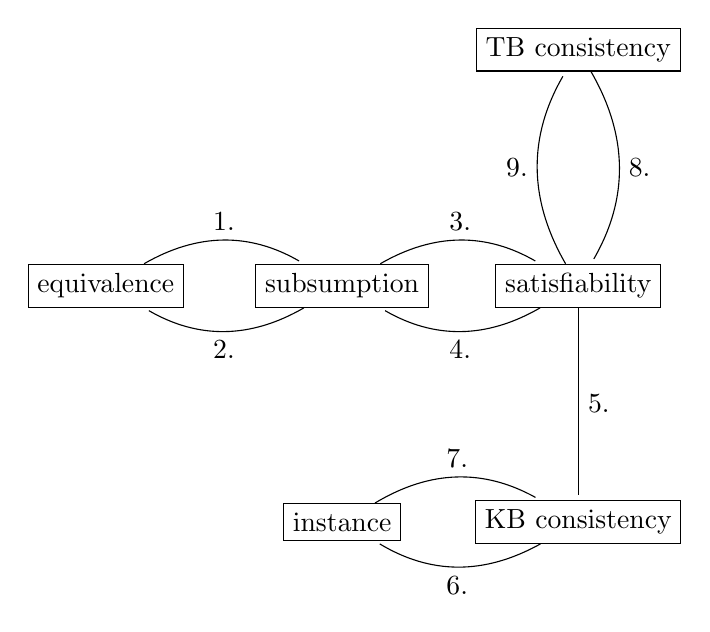
\begin{tikzpicture}[align=center,node distance=3cm, shorten >= 2pt]
		\node[draw] (eq) {equivalence};
		\node[draw, right of = eq] (sub) {subsumption};
		\node[draw, right of = sub] (sat) {satisfiability};
		\node[draw, below of = sat] (kbc) {KB consistency};
		\node[draw, left of = kbc] (ins) {instance};
		\node[draw, above of = sat] (tbc) {TB consistency};
		\draw (eq) edge[above, bend left] node{1.} (sub);
		\draw (sub) edge[below, bend left] node{2.} (eq);
		\draw (sub) edge[above, bend left] node{3.} (sat);
		\draw (sat) edge[below, bend left] node{4.} (sub);
		\draw (sat) edge[right]  node{5.} (kbc);
		\draw (kbc) edge[below, bend left] node{6.} (ins);
		\draw (ins) edge[above, bend left] node{7.} (kbc);
		\draw (tbc) edge[right, bend left] node{8.} (sat);
		\draw (sat) edge[left, bend left] node{9.} (tbc);
	\end{tikzpicture}
	\caption{Polynomial reductions between decision problems.}
	\label{fig:problem reductions}
\end{figure}
\begin{note}
	These reductions do not only hold for $\mathcal{ALC}$, but for all DLs with the constructors negation and conjunction.
	The last one also needs an existential quantifier.
	They correspond to the following lemma:
\end{note}

\begin{theorem}[polynomial reductions]
	Let $\mathcal{K} = \left( \mathcal{T}, \mathcal{A} \right)$ be a knowledge base, 
	$C, D$ concept descriptions and $a \in \mathscr{I}$.
	\begin{enumerate}
		\item $C \equiv_{\mathcal{T}} D \iff C \sqsubseteq_{\mathcal{T}} D \land D \sqsubseteq_{\mathcal{T}} C$ 
		\item $C \sqsubseteq_{\mathcal{T}} D \iff C \equiv_{\mathcal{T}} C \sqcap D$
		\item $C \sqsubseteq_{\mathcal{T}} D \iff C \sqcap \neg D$ is unsatisfiable w.r.t.\ $\mathcal{T}$
		\item $C$ is satisfiable w.r.t.\ $\mathcal{T} \iff C \not\sqsubseteq_{\mathcal{T}} \bot$
		\item $C$ is satisfiable w.r.t.\ $\mathcal{T} \iff \left( \mathcal{T}, \left\{ a:C \right\} \right)$ is consistent
		\item $a$ is an instance of $C$ w.r.t.\ $\mathcal{K} \iff \left( \mathcal{T}, \mathcal{A} \cup \left\{ a: \neg C \right\} \right)$ is inconsistent
		\item $\mathcal{K}$ is consistent $\iff a$ is not an instance of $\bot$ w.r.t.\ $\mathcal{K}$
		\item $\mathcal{T}$ is consistent $\iff \top$ is satisfiable w.r.t.\ $\mathcal{T}$
		\item $C$ is satisfiable w.r.t.\ $\mathcal{T} \iff \mathcal{T} \cup \left\{ \top \sqsubseteq \exists r.C \right\}$,
			where $r$ is a new role that does not occur in $C$ or $\mathcal{T}$,
			is consistent.
	\end{enumerate}
\end{theorem}
\begin{proof}
	\begin{enumerate}
		\item By definition.
		\item An easy consequence of the set inclusion relation $\subseteq$.
		\item
			\begin{align*}
				C \sqsubseteq_{\mathcal{T}} D & \iff \forall \mathcal{I}, \mathcal{I} \vDash \mathcal{T}: C^{\mathcal{I}} \subseteq D^{\mathcal{I}}\\
											  & \iff \forall \mathcal{I}, \mathcal{I} \vDash \mathcal{T} : C^\mathcal{I} \cap (\Delta^{\mathcal{I}} \setminus D^{\mathcal{I}}) = \emptyset\\
											  & \iff \forall \mathcal{I}, \mathcal{I} \vDash \mathcal{T}: C^{\mathcal{I}} \cap (\neg D)^\mathcal{I} = \emptyset\\
											  & \iff \forall \mathcal{I}, \mathcal{I} \vDash \mathcal{T}: \left( C \sqcap \neg D \right)^\mathcal{I} = \emptyset\\
											  & \iff \left( C \sqcap \neg D \right) \text{is unsatisfiable w.r.t.}\ \mathcal{T} 
			\end{align*}
		\item trivial.
		\item see lecture video.
		\item "$ \implies$": By its contraposition. \newline
			Assume that $\left( \mathcal{T}, \mathcal{A} \cup \left\{a: \neg C \right\} \right)$ is indeed consistent.
			Then there is  a model $\mathcal{I}$ of $\mathcal{T} , \mathcal{A}$ and $\left\{ a: \neg C \right\}$.
			But then $\mathcal{I}$ is a model of $\mathcal{K} = \left( \mathcal{T}, \mathcal{A} \right)$ such that
			$a^{\mathcal{I}} \notin C^\mathcal{I}$.
			Thus, $a$ is not an instance of $C$ w.r.t.\ $\mathcal{K}$. \newline
			"$\impliedby$": Also by its contraposition. \newline
			Assume that $a$ in not an instance of $C$ w.r.t.\ $\mathcal{K}$.
			Thus there is a model $\mathcal{I}$ of $\mathcal{K}$ with $a^\mathcal{I} \notin C^\mathcal{I}$.
			Thus, $\mathcal{I}$ is a model of $\left( \mathcal{T}, \mathcal{A} \cup \left\{ a: \neg C \right\} \right)$.
		\item By the contraposition: \newline
			Assume that $\mathcal{K}$ is consistent and let $\mathcal{I}$ be a model of $\mathcal{K}$.
			Then $a^\mathcal{I} \notin \emptyset = \bot^\mathcal{I}$.
			If $\mathcal{K}$ is inconsistent, then there is no model of $\mathcal{K}$.
			Thus $a^{\mathcal{I}} \in \bot^\mathcal{I}$ holds in all models since there are none.
		\item see lecture video.
		\item "$ \implies$": \newline
			Assume that $\mathcal{I}$ is a model of $\mathcal{T}$ such that $C^\mathcal{I} \neq \emptyset$
			(definition of satisfiability).
			Let $d \in C^{\mathcal{I}}$.
			We extend $\mathcal{I}$ to $\mathcal{I}'$by setting $r^{\mathcal{I}} = \left\{ (e,d) \mid  e \in \Delta^{\mathcal{I}} \right\}$.
			Since $r$ does not occur in $C$ or $\mathcal{T}$, we still have $d \in C^\mathcal{I'}$ and $\mathcal{I'}$ is a model of $\mathcal{T}$. \newline
			"$\impliedby$": \newline
			If $\mathcal{I}$ is a model of $\mathcal{T} \cup \left\{ \top \sqsubseteq \exists r.C \right\}$,
			then let $e$ be an arbitrary element of $\Delta^{\mathcal{I}}$.
			Then $e \in \left( \exists r.C \right)^{\mathcal{I}}$, and thus there is an $d \in \Delta^{\mathcal{I}}$ 
			with $\left( e,d \right) \in r^{\mathcal{I}}$ and $d \in C^\mathcal{I}$.
			Thus, $C$ is satisfiable w.r.t.\ $\mathcal{T}$.
			\qedhere
	\end{enumerate}
\end{proof}

Now we will show, that satisfiability w.r.t.\ $\mathcal{T}$ can be reduced to satisfiability (without $\mathcal{T}$) and
Knowledge base consistency can be reduced to ABox consistency.
However this reduction is in general not possible in polynomial time.

\begin{prop}[reductions to ABox consistency]
Let  $\mathcal{K} = (\mathcal{T}, \mathcal{A})$ be a knowledge base, where $\mathcal{T}$ is acyclic, and $C$ a concept description.
The expanded versions $\widehat{C}$ and $\widehat{A}$ of $C$ and $A$ w.r.t.\ $\mathcal{T}$ are obtained by
replacing all defined concepts occurring in $C$ and $A$ by their definitions in the expanded version $\widehat{\mathcal{T}}$ of $\mathcal{T}$.
Then:
	\begin{enumerate}
		\item $C$ is satisfiable w.r.t.\ $\mathcal{T} \iff \widehat{C}$ is satisfiable.
		\item $\mathcal{K} = (\mathcal{T},\mathcal{A})$ is consistent $\iff (\emptyset,\widehat{\mathcal{A}}$) is consistent.
	\end{enumerate}
\end{prop}
\begin{merke}[frametitle=Important Note:]
	The problem of deciding whether $(\emptyset, \widehat{\mathcal{A}})$ is consistent is also called "ABox consistency".
	The proposition above shows, that each of the decision problems discussed before can be reduce to ABox consistency,
	as long as no cyclic TBox is involved.
\end{merke}
\begin{proof}
	\begin{enumerate}
		\item " $\implies$":\newline
			Let $\mathcal{I}$ be a model of $\mathcal{T}$ with $C^\mathcal{I} \neq \emptyset$.
			Then $\mathcal{I}$ is also a model of $\widehat{\mathcal{T}}$ and we have $\emptyset \neq C^\mathcal{I} = \widehat{C}^\mathcal{I}$.
			Thus, $\widehat{C}$ is satisfiable. \newline
			"$\impliedby$": \newline
			Let $\mathcal{I}$ be an interpretation with $\widehat{C}^{\mathcal{I}} \neq \emptyset$.
			Let $\mathcal{J}$ be the primitive interpretation of which $\mathcal{I}$ is an extension
			and let $\mathcal{I}'$ be the model of $\mathcal{T}$ that extends $\mathcal{J}$.
			Since $\widehat{C}$ contains only primitive concepts,
			we have $\emptyset \neq \widehat{C}^{\mathcal{I}} = \widehat{C}^\mathcal{J} = \widehat{C}^{\mathcal{I'}} = C^{\mathcal{I'}}$,
			since $\mathcal{I}'$ is a model of $\mathcal{T}$ and $\widehat{\mathcal{T}}$.
		\item similar
			\qedhere
	\end{enumerate}
\end{proof}
\newpage

	\lecture{5}{27.04.2021}{}
So as long as we are not interested in the efficiency of reasoning, we do not need to develop reasoning procedures for TBoxes.
However, this reduction is in general not polynomial, since the expanded versions may be exponential in the size of $\mathcal{T}$.
One can easily see this with the following example on a TBox:
\begin{align*}
	A_0 &\equiv \forall r.A_1 \sqcap \forall s. A_1 \\
	A_1 &\equiv \forall r.A_2 \sqcap \forall s.A_2 \\
	\vdots & \\
	A_{n-1} & \equiv \forall r.A_n \sqcap \forall s.A_{n}
\end{align*}
The size of this TBox is linear in $n$,
but the expansion version $\widehat{A}_0$ of $A_0$ contains $A_n$ $2^n$ times.

\subsection{Relationship with FOL}
Like everything so far, reasoning in $\mathcal{ALC}$ can be translated into reasoning in FOL:
\begin{lemma}
	Let $\mathcal{K} = ( \mathcal{T},\mathcal{A})$ be a knowledge base, $C,D$ concept descriptions and $a$ an individual name.
	\begin{enumerate}
		\item $C \sqsubseteq_{\mathcal{T}} D \iff \tau(\mathcal{T}) \vDash \forall x.(\tau_x(C)(x) \Rightarrow \tau_x(D)(x))$
		\item $ \mathcal{K}$ is consistent $ \iff \tau(\mathcal{K})$ is consistent
		\item $a$ is an instance of $C$ w.r.t.\ $\mathcal{K} \iff \tau \left( \mathcal{K} \right) \vDash \tau_x(C)(a)$
	\end{enumerate}
\end{lemma}

\begin{proof}
	Exercise!	
\end{proof}

\newpage
\section{Further problems}
So far we have seen the basics of the $\mathcal{ALC}$-DL system and its inference problems.
Often times it is not sufficient to just know \textit{if} one concept is subsumed by another,
but which concepts are actually subsumed by which.
\textbf{Classification} is the task to compute the subsumption hierarchy of \textit{all} concept names occurring in the TBox.
\newline
Likewise, it could be of interest to know, which is the most specific concept name in the TBox to which an ABox individual belongs.
This problem is called \textbf{Realization}.
\newline
Therefore DL-systems often include solution procedures for these problems.

\section{Further relationships with FOL}
We will now introduce a new constructor for illustrative purposes.
If $r$ is a role name and $C$ is a concept description, then $\exists r^+.C $
is a concept description, with the semantics
\begin{align*}
	\begin{split}
		(\exists r^+.C)^\mathcal{I} \coloneqq &\left\{ d \in \Delta^{\mathcal{I}} \mid \exists n \geq 1, \exists d_1,\cdots, d_n \in \Delta^\mathcal{I} : \right.\\
											  &\left. (d,d_1) \in r^\mathcal{I}, \cdots, (d_{n-1},d_n) \in r^\mathcal{I} \land d_n \in C^\mathcal{I}\right\}
	\end{split}
\end{align*}

We claim, that $\exists r^+.C$ cannot be expressed in $\mathcal{ALC}$.
\begin{proof}
	Assume that there is an $\mathcal{ALC}$ concept $D$ such that $D \equiv \exists r^+.C$.
	Consider the ABox $\mathcal{A} = \left\{ a:D \right\}$.
	Let $ \mathcal{B} = \left\{ a : \forall r.\neg C, a: \forall r.\forall r.\neg C, a:\forall r.\forall r.\forall r.\neg C,\ldots \right\}$.
	Then $\mathcal{A} \cup \mathcal{B}$ is inconsistent.
	Since $\mathcal{A} \cup \mathcal{B}$ can be translated to FOL, compactness applies, i.e.,
	there is a finite subset $\mathcal{C} \subseteq \mathcal{A} \cup \mathcal{B}$ such that $\mathcal{C}$ is inconsistent.
	Let $n$ be the maximal nesting of value-restrictions in $\mathcal{C}$, i.e.,
	$\mathcal{C}$ does not contain $\underbrace{\forall r. \forall r. \ldots \forall r.}_{n+1} \neg C$.
	But then there obviously is a model of $\mathcal{C}$. $\contra$
\end{proof}
This shows, that certain concepts can be expressed in FOL, but not in $\mathcal{ALC}$.

\chapter{A Little Bit of Model Theory}
Like we already saw, interpretations of $\mathcal{ALC}$ can be viewed as graphs.
We introduce the notion of bisimulation between graphs and therefore between interpretations.
We will then show, that $\mathcal{ALC}$-concepts cannot distinguish bisimular nodes.
Afterwards these results will grant us the power to show restrictions of the expressive power of $\mathcal{ALC}$ and
interesting properties of models of $\mathcal{ALC}$:
\begin{itemize}
	\item tree model property
	\item closure under disjoint union
\end{itemize}
Furthermore we will show the very important property of $\mathcal{ALC}$: the finite model property.

\section{Bisimulation}
\begin{definition}[Bisimulation]\label{def:bisimulation}
	Let $\mathcal{I}_1$ and $\mathcal{I}_2$ be interpretations.
	The relation $\rho \subseteq \Delta^{\mathcal{I}_{1}} \times \Delta^{\mathcal{I}_2}$ is a bisimulation between $\mathcal{I}_1$ and $\mathcal{I}_2$ iff:
	\begin{enumerate}[label=(\roman*)]
		\item $d_1 \rho d_2 \implies d_1 \in A^{\mathcal{I}_1} \text{ iff } d_2 \in A^{\mathcal{I}_2}$ for all $A \in \mathscr{C}$
		\item $d_1 \rho d_2 \land  (d_1, d_1') \in r^{\mathcal{I}_1}$ implies the existence of $d_2' \in \Delta^{\mathcal{I}_2}$ such that
			$d_1' \rho d_2' \land (d_2, d_2') \in r^{\mathcal{I}_2}$ for all $r \in \mathscr{R}$
		\item $d_1 \rho d_2 \land  (d_2, d_2') \in r^{\mathcal{I}_2}$ implies the existence of $d_1' \in \Delta^{\mathcal{I}_1}$ such that
			$d_1' \rho d_2' \land (d_1, d_1') \in r^{\mathcal{I}_1}$ for all $r \in \mathscr{R}$
	\end{enumerate}
\end{definition}

\begin{note}
	\begin{itemize}
		\item $\mathcal{I}_1 = \mathcal{I}_2$ is possible
		\item the empty relation $\emptyset$ is always a bisimulation.
	\end{itemize}
\end{note}

\begin{notation}
	Let $\mathcal{I}_1, \mathcal{I}_2$ be interpretations and $d_1 \in \Delta^{\mathcal{I}_1}, d_2 \in \Delta^{\mathcal{I}_2}$.
	We then write:
	\[
		\left( \mathcal{I}_1, d_1 \right) \sim \left( \mathcal{I}_2, d_2 \right) \iff \exists \text{ a bisimulation $\rho$ between  $\mathcal{I}_1, \mathcal{I}_2$
		such that $d_1 \rho d_2$}
	.\]
	And we say "$d_1$ in $\mathcal{I}_1$ is bisimular to $d_2$ in $\mathcal{I}_2$".
\end{notation}

\begin{theorem}[Bisimulation invariance of $\mathcal{ALC}$]\label{thm: bisimulation invariance}
	If $ \left( \mathcal{I}_1,d_1 \right) \sim \left( \mathcal{I}_2, d_2 \right)$, then the following holds for all $\mathcal{ALC}$-concepts $C$ :
	\[
		d_1 \in C^{\mathcal{I}_1} \iff d_2 \in C^{\mathcal{I}_2}
	.\]
\end{theorem}
This theorem essentially tells us, that $\mathcal{ALC}$-concepts cannot distinguish between bisimular elements.

	\lecture{6}{29.04.2021}{}

\begin{proof}
	By induction on the structure of $C$ :
	\begin{itemize}
		\item $C = A \in \mathscr{C}$:
			Then $d_1 \in A^{\mathcal{I}_1}$ iff $d_2 \in A^{\mathcal{I}_2}$ is an immediate consequence of $d_1 \rho d_2$ for a bisimulation $\rho$.
		\item $C = D \sqcap E$ :
			$d_1 \in \left( D \sqcap E \right)^{\mathcal{I}_1}$ iff $d_1 \in D^{\mathcal{I}_1}$ and $d_1 \in E^{\mathcal{I}_1}$.
			But then $d_2 \in D^{\mathcal{I}_2}$ and $d_2 \in E^{\mathcal{I}_2}$ (induction).
			And therefore $d_2 \in \left( D \sqcap E \right)^{\mathcal{I}_2}$.
		\item $\neg, \sqcup$ can be treated similarly.
		\item $C = \exists r.D$ :
				$d_1 \in \left( \exists r.D \right)^{\mathcal{I}_1}$ iff there is $d_1' \in \Delta^{\mathcal{I}_1}$ such that $(d_1, d_1') \in r^{\mathcal{I}_1}$ and $d_1' \in D^{\mathcal{I}_1}$.
				Then there is $d_2' \in \Delta^{\mathcal{I}_2}$ such that $\left( d_2, d_2' \right) \in r^{\mathcal{I}_2}$ and $d_1' \rho d_2'$.
				By induction we get that $d_2' \in D^{\mathcal{I}_2}$ and therefore  $d_2 \in \left( \exists r.D \right)^{\mathcal{I}_2}$.
			\item $C = \forall r.D$ can be treated similarly.
	\end{itemize}
\end{proof}

\section{Expressive power}
We have so far introduced extensions of $\mathcal{ALC}$ by concept constructors \textbf{number restrictions}, \textbf{nominals} and the role constructor \textbf{invers roles}.
We will now show, that they really extend $\mathcal{ALC}$, i.e., there is no way these could be expressed by plain $\mathcal{ALC}$.

\begin{prop}[$\mathcal{ALCN}$ is more expressive than $\mathcal{ALC}$]
	No $\mathcal{ALC}$-concept description is equivalent to the $\mathcal{ALCN}$-concept description $\left( \leq 1 r \right)$.
\end{prop}
\begin{proof}
	Assume that $C$ is an $\mathcal{ALC}$-concept description such that $C \equiv ( \leq 1 r )$, i.e.\ $C^{\mathcal{I}} = \left( \leq 1 r \right)^\mathcal{I}$ holds for all interpretations $\mathcal{I}$.
	Consider the following two interpretations $\mathcal{I}_1$ and $\mathcal{I}_2$ :
	\begin{figure}[H]
		\centering
		\begin{subfigure}[t]{.475\textwidth}
			\centering
			\begin{tikzpicture}
				\node[default] (d1) {$d_1$};
				\node[default, below of = d1] (e1) {$e_1$};
				\draw (d1) edge[left] node{$r$} (e1);
			\end{tikzpicture}
			\caption{$\mathcal{I}_1$}
		\end{subfigure}
		\hfill
		\begin{subfigure}[t]{.475\textwidth}
			\centering
			\begin{tikzpicture}
				\node[default] (d2) {$d_2$};
				\node[default, below left of = d2] (e21) {$e_{2,1}$};
				\node[default, below right of = d2] (e22) {$e_{2,2}$};
				\draw (d2) edge[left] node{$r$} (e21);
				\draw (d2) edge[right] node{$r$} (e22);
			\end{tikzpicture}
			\caption{$\mathcal{I}_2$}
		\end{subfigure}
	\end{figure}
	Then $\rho \coloneqq \left\{ (d_1,d_2), (e_1,e_{2,1}), (e_1,e_{2,2}) \right\}$ is a bisimulation, which shows $(\mathcal{I}_1, d_1) \sim (\mathcal{I}_2,d_2)$.
	Thus, we have $d_1 \in C^{\mathcal{I}_1} \iff d_2 \in C^{\mathcal{I}_2}$.
	This yields a contradiction, since $d_1 \in ( \leq 1r)^{\mathcal{I}_1} = C^{\mathcal{I}_1}$ but $d_2 \notin ( \leq 1r)^{\mathcal{I}_2} = C^{\mathcal{I}_2}$. $\contra$
\end{proof}

\begin{prop}[$\mathcal{ALCI}$ is more expressive than $\mathcal{ALC}$]
	No $\mathcal{ALC}$-concept description is equivalent to the $\mathcal{ALCI}$-concept description $\exists r^{-}.\top$.
\end{prop}
\begin{proof}
	Assume that $C$ is an $\mathcal{ALC}$-concept description such that $C \equiv \exists r^{-}.\top$.
	Consider the following two interpretations:
	\begin{figure}[H]
		\centering
		\begin{subfigure}[t]{.475\textwidth}
			\centering
			\begin{tikzpicture}
				\node[default] (e1) {$e_1$};
				\node[default, below of = e1] (d1) {$d_1$};
				\draw (e1) edge[left] node{$r$} (d1);
			\end{tikzpicture}
			\caption{$\mathcal{I}_1$}
		\end{subfigure}
		\hfill
		\begin{subfigure}[t]{.475\textwidth}
			\centering
			\begin{tikzpicture}
				\node[default] (d2) {$d_2$};
			\end{tikzpicture}
			\caption{$\mathcal{I}_2$}
		\end{subfigure}
	\end{figure}
	Then $\rho \coloneqq \left\{ (d_1,d_2) \right\}$ is a bisimulation, which shows $\left(  \mathcal{I}_1, d_1 \right) \sim \left( \mathcal{I}_2,d_2 \right)$.
	Thus, we have  $d_1 \in C^{\mathcal{I}_1} \iff d_2 \in C^{\mathcal{I}_2}$.
	This yields a contradiction, since $d_1 \in \left( \exists r^{-}.\top \right)^{\mathcal{I}_1} = C^{\mathcal{I}_1}$, but
	$d_2 \notin \left( \exists r^{-}.\top \right)^{\mathcal{I}_2} = C^{\mathcal{I}_2}$. $\contra$
\end{proof}

\begin{prop}[$\mathcal{ALCO}$ is more expressive than $\mathcal{ALC}$]
	No $\mathcal{ALC}$-concept description is equivalent to the $\mathcal{ALCO}$-concept description $\left\{ a \right\}$.
\end{prop}
\begin{proof}
	Assume that $C$ is an $\mathcal{ALC}$-concept description such that $C \equiv \left\{ a \right\}$.
	Consider the following two interpretations:
	\begin{figure}[H]
		\centering
		\begin{subfigure}[t]{.475\textwidth}
			\centering
			\begin{tikzpicture}
				\node[default, label =left: $\left\{ a \right\}^{\mathcal{I}_1}$] (d1) {$d_1$};
			\end{tikzpicture}
			\caption{$\mathcal{I}_1$}
		\end{subfigure}
		\hfill
		\begin{subfigure}[t]{.475\textwidth}
			\centering
			\begin{tikzpicture}
				\node[default] (d2) {$d_2$};
				\node[default, label= right: $\left\{ a \right\}^{\mathcal{I}_2}$, right of = d2] (e2) {$e_2$};
			\end{tikzpicture}
			\caption{$\mathcal{I}_2$}
	\end{subfigure}
	\end{figure}
	The meaning of these interpretations is, that $a^{\mathcal{I}_1} = d_1$ and $a^{\mathcal{I}_2} = e_2$.
	Then $\rho \coloneqq \left\{ (d_1,d_2) \right\}$ is a bisimulation, which yields $\left( \mathcal{I}_1, d_1 \right) \sim \left( \mathcal{I}_2, d_2 \right)$.
	Thus, $d_1 \in C^{\mathcal{I}_1} \iff d_2 \in C^{\mathcal{I}_2}$.
	This yields a contradiction, since $d_1 \in \left\{ a \right\}^{\mathcal{I}_1} = C^{\mathcal{I}_1}$, but
	 $d_2 \notin \left\{ a \right\}^{\mathcal{I}_2} = C^{\mathcal{I}_2}$. $\contra$
\end{proof}
These proofs were the result of the fact, that we defined bisimulation with $\mathcal{ALC}$ in mind.
One could also define a notion of bisimulation under which $\mathcal{ALCN}$, $\mathcal{ALCI}$ or $\mathcal{ALCO}$ are invariant.

\section{Closure under disjoint union}
We will now introduce the notion of disjoint union for interpretations.
This will enable us to combine multiple interpretations into a bigger one, containing the interpretations it was built from,
but no interaction between them.
\begin{definition}
	Let $\mathfrak{R}$ be an index set and $\left( \mathcal{I}_{\nu} \right)_{\nu \in \mathfrak{R}}$ a family of interpretations $\mathcal{I}_{\nu} = \left( \Delta^{\mathcal{I}_{\nu}}, \cdot^{\mathcal{I}_{\nu}} \right)$.
	Their disjoint union $\mathcal{J}$ is defined as follows:
	\begin{align*}
		\Delta^{\mathcal{J}} &= \left\{ (d,\nu) \mid \nu \in \mathfrak{R}\land d \in \Delta^{\mathcal{I}_{\nu}} \right\}, \\
		A^{\mathcal{J}} &= \left\{ (d,\nu) \mid \nu \in \mathfrak{R} \land d \in A^{\mathcal{I}_\nu}\right\} \text{for all } A \in \mathscr{C}, \\
		r^{\mathcal{J}} &= \left\{ \left( (d,\nu),(e,\nu) \right) \mid \nu \in \mathfrak{R} \land (d,e) \in r^{\mathcal{I}_\nu} \right\} \text{for all } r \in \mathscr{R}.
	\end{align*}
\end{definition}
\begin{notation}
	We then write
	\[
	\mathcal{J} = \biguplus_{\nu \in \mathfrak{R}} \mathcal{I}_{\nu}
	.\]
\end{notation}
\begin{note}
	If there are some $\Delta^{\mathcal{I}_{\nu_1}}, \Delta^{\mathcal{I}_{\nu_2}}$ that are not disjoint,
	we make them artificially disjoint by adding the index $\nu$ to the tuple.
\end{note}

\begin{lemma}\label{lemma:disjoint union 1}
	For $\nu \in \mathfrak{R}$, all $\mathcal{ALC}$-concept description $C$, and all $d \in \Delta^{\mathcal{I}_\nu}$ we have:
	\[
		d \in C^{\mathcal{I}_\nu} \iff (d,\nu) \in C^{\mathcal{J}}
	,\]
	where $\mathcal{J} = \biguplus_{\nu \in \mathfrak{R}} \mathcal{I}_{\nu}$.
\end{lemma}
\begin{proof}[Proof sketch]
	Let $\mathcal{J} = \biguplus_{\nu \in \mathfrak{R}} \mathcal{I}_\nu$.
	We claim that
	\[
	\rho_\nu \coloneqq \left\{ \left( (d,\nu),d \right) \mid d \in \Delta^{\mathcal{I}_\nu} \right\}
	\]
	is a bisimulation (and proof that).
	And then lemma \ref{lemma:disjoint union 1} follows from theorem \ref{thm: bisimulation invariance}.
\end{proof}

\begin{theorem}\label{thm:disjoint union closure}
	Let $\mathcal{T}$ be an $\mathcal{ALC}$ TBox and $(\mathcal{I}_\nu)_{\nu \in \mathfrak{R}}$ a family of models of $\mathcal{T}$.
	Then its disjoint union $\mathcal{J} = \biguplus_{\nu \in \mathfrak{R}} \mathcal{I}_\nu$ is also a model of $\mathcal{T}$.
\end{theorem}
This theorem tells us, that models of TBoxes are closed under disjoint union.
\begin{proof}
	Let $C \sqsubseteq D \in \mathcal{T}$.
	We must show that $C^{\mathcal{J}} \subseteq D^{\mathcal{J}}$.
	Let $\left( d,\nu \right) \in C^{\mathcal{J}}$.
	By lemma \ref{lemma:disjoint union 1}, this implies $d \in C^{\mathcal{I}_\nu}$.
	Since $\mathcal{I}_\nu$ is a model of $\mathcal{T}$, we obtain $d \in D^{\mathcal{I}_\nu}$.
	Again, by lemma \ref{lemma:disjoint union 1}, this implies $(d,\nu) \in D^{\mathcal{J}}$.
\end{proof}

\begin{corollary}
 	Let $\mathcal{T}$ be an $\mathcal{ALC}$ TBox and $C$ an $\mathcal{ALC}$ concept that is satisfiable w.r.t.\ $\mathcal{T}$.
	Then there is a model $\mathcal{J}$ of $\mathcal{T}$ in which the extension $C^{\mathcal{J}}$ of $C$ is infinite.
\end{corollary}
\begin{proof}
	Since $C$ is satisfiable w.r.t.\ $\mathcal{T}$, there is a model $\mathcal{I}$ of $\mathcal{T}$ and $d \in \Delta^{\mathcal{I}}$ such that $d \in C^{\mathcal{I}}$.
	For $\nu \in \N^{+}$ let $\mathcal{I}_\nu = \mathcal{I}$.
	Let $\mathcal{J} = \biguplus_{\nu \geq 1} \mathcal{I}_\nu$.
	We know that $\mathcal{J}$ is a model of $\mathcal{T}$ since $\mathcal{I}$ is a model of $\mathcal{T}$ (theorem \ref{thm:disjoint union closure}).
	In $\mathcal{J}$, $C$ has infinitely many elements, since $(d,\nu) \in C^{\mathcal{J}}$ for $\nu \geq 1$.
\end{proof}
Therefore the only concepts that are \textbf{always} interpreted as a finite set,
are unsatisfiable concepts (w.r.t.\ a TBox $\mathcal{T}$).
As long as a concept is satisfiable one can find arbitrarily large interpretations for it.
In other words: $\mathcal{ALC}$ can not express the finiteness of concepts.

\section{Finite model property}
\begin{definition}[Finite model]
	The interpretation $\mathcal{I}$ is called a model of a concept $C$ w.r.t.\ a TBox $\mathcal{T}$,
	if $\mathcal{I}$ is a model of $\mathcal{T}$ such that $C^{\mathcal{I}} \neq \emptyset$.
	We call this model finite if $\Delta^{\mathcal{I}}$ is finite.
	\newline
	We call the following the \textit{Finite model property} (of $\mathcal{ALC}$):
	\newline
	If $\mathcal{T}$ is an $\mathcal{ALC}$-TBox and $C$ an $\mathcal{ALC}$-concept description 
	such that $C$ is satisfiable w.r.t.\ $\mathcal{T}$,
	then $C$ has a finite model w.r.t.\ $\mathcal{T}$.
\end{definition}	
To proof this we first need some auxiliary results.
Actually, we will even show something stronger, namely, that $\mathcal{ALC}$ has the bounded model property.
To do so, we need a notion of the size of $\mathcal{ALC}$-concepts.

\begin{mdframed}[frametitle={Sizes in $\mathcal{ALC}$}]
	We define the size of an $\mathcal{ALC}$-concept description recursively:
	\begin{itemize}
		\item $C = A \in \mathscr{C}$: $\func{size}(C) \coloneqq 1$,
		\item $C = C_1 \sqcap C_2$ or $C = C_1 \sqcup C_2$: $\func{size}(C) \coloneqq 1 + \func{size}(C_1) + \func{size}(C_2)$,
		\item $C = \neg D$ or $C = \exists r.D$ or $C = \forall r.D$: $\func{size}(C) \coloneqq 1 + \func{size}(D)$.
	\end{itemize}
	We also define the size of a TBox $\mathcal{T}$ as follows:
	\[
		\func{size}(\mathcal{T}) \coloneqq \sum_{C \sqsubseteq D \in \mathcal{T}} \func{size}(C) + \func{size}(D)
	.\]
\end{mdframed}

\begin{mdframed}[frametitle={Subconcepts in $\mathcal{ALC}$}]
	We define the subconcepts of an $\mathcal{ALC}$-concept description recursively:
	\begin{itemize}
		\item $C = A \in \mathscr{C}$ : $\func{sub}(C) \coloneqq \left\{ A \right\}$,
		\item $C = C_1 \sqcap C_2$ or $C = C_1 \sqcup C_2$ : $\func{sub}(C) \coloneqq \left\{ C \right\} \cup \func{sub}(C_1) \cup \func{sub}(C_2)$,
		\item $C = \neg D$ or $C = \exists r.D$ or $C = \forall r.D$ : $\func{sub}(C) \coloneqq \left\{ C \right\} \cup \func{sub}(D)$.
	\end{itemize}
	We also define the subconcepts of a TBox $\mathcal{T}$ as follows:
	\[
		\func{sub}(\mathcal{T}) \coloneqq \bigcup_{C \sqsubseteq D \in \mathcal{T}} \func{sub}(C) \cup \func{sub}(D)
	.\]
\end{mdframed}
\begin{note}
	Subconcepts are only the syntactic building blocks of a concept, \textbf{not} the concepts subsumed by it.
\end{note}

	\lecture{7}{04.05.2021}{}

\begin{lemma}
	For arbitrary concept descriptions $C$ and arbitrary TBoxes $ \mathcal{T}$ the following hold:
	\begin{itemize}
		\item $\left| \text{sub}(C) \right| \leq \text{size}(C)$ 
		\item $\left| \text{sub}(\mathcal{T}) \right| \leq \text{size}(\mathcal{T})$
	\end{itemize}
\end{lemma}

	\lecture{8}{06.05.2021}{}
\begin{proof}
	By definition of the extension of concept names in $\mathcal{J}$, we have that
	\[
		p \in A^{\mathcal{J}} \iff \func{end}(p) \in A^{\mathcal{I}}
	.\]
	Thus, condition (i) in definition \ref{def:bisimulation} is satisfied.

	To show that condition (ii) of definition \ref{def:bisimulation} is satisfied, 
	we assume $(p,e) \in \rho$ and $(p,p') \in r^\mathcal{J}$.
	Since $\func{end}(p)$ is the only element in $\Delta^{\mathcal{I}}$, that is $\rho$-related to $p$,
	we have $e = \func{end}(p)$.
	We must show that there is a $f \in \Delta^{\mathcal{I}}$ such that $(p',f) \in \rho$ and $(e,f) \in r^{\mathcal{I}}$.
	We define $f = \func{end}(p')$.
	We know that then $(p',f) \in \rho$.
	Thus, it remains to show, that $(\func{end}(p),\func{end}(p')) \in r^{\mathcal{I}}$.
	This is an immediate consequence of the definition of $r^{\mathcal{J}}$:

	To show that condition (iii) of definition \ref{def:bisimulation} is satisfied,
	we assume $(p,e) \in \rho$ and $(e,f) \in r^{\mathcal{I}}$.
	We must find a path $p'$ such that $(p',f) \in \rho$ and $(p,p') \in r^{\mathcal{J}}$.
	We define $p' \coloneqq p,f$.
	This is indeed a $d$-path, since $p$ is a $d$-path with $\func{end}(p) = e$ 
	and $(e,f) \in r^{\mathcal{I}}$.
	In addition, $\func{end}(p') = f$, which shows $(p',f) \in \rho$.
	Finally, we have $p' = p,\func{end}(p')$ and $(\func{end}(p), \func{end}(p')) \in r^\mathcal{I}$.
	This yields $(p,p') \in r^\mathcal{J}$.
\end{proof}

\begin{prop}\label{prop:tree model invariance}
	For all $\mathcal{ALC}$-concepts $C$ and $p \in \Delta^{\mathcal{J}}$ we have
	\[
		p \in C^{\mathcal{J}} \iff \func{end}(p) \in C^{\mathcal{I}}
	.\]
\end{prop}
This is just the bisimulation invariance of $\mathcal{ALC}$ in this special case.

\begin{theorem}[tree model property]\label{tree model property}
	$\mathcal{ALC}$ has the tree model property,
	i.e.\ if $\mathcal{T}$ is an $\mathcal{ALC}$-TBox and $C$ an $\mathcal{ALC}$-concept description
	such that $C$ is satisfiable w.r.t.\ $\mathcal{T}$, then $C$ has a tree model w.r.t.\ $\mathcal{T}$.
\end{theorem}
\begin{note}
	$\mathcal{ALC}$ does however not have the finite tree model property.
\end{note}
\begin{proof}
	Let $\mathcal{I}$ be an interpretation such that $\mathcal{I}$ is a model of $\mathcal{T}$ and $d \in C^{\mathcal{I}}$.
	We show that the unraveling $\mathcal{J}$ of $\mathcal{I}$ at $d$ is a tree model of $C$ w.r.t.\ $\mathcal{T}$.
	\begin{enumerate}
		\item To prove that $\mathcal{J}$ is a model of $\mathcal{T}$,
			consider a GCI $D \sqsubseteq E$ in $\mathcal{T}$.
			Assume that $p \in D^{\mathcal{J}}$.
			We must then show $p \in E^{\mathcal{J}}$.
			By proposition \ref{prop:tree model invariance},
			we know that $\func{end}(p) \in D^{\mathcal{I}}$.
			Then $\func{end}(p) \in E^{\mathcal{I}}$, since $\mathcal{I}$ is a model of $\mathcal{T}$.
			We can apply proposition \ref{prop:tree model invariance} again to obtain $p \in E^{\mathcal{J}}$.
		\item We show that  the graph
			\[
				\mathcal{G}_{\mathcal{J}} = \left( \Delta^{\mathcal{J}}, \bigcup_{r \in \mathscr{R}} r^{\mathcal{J}} \right)
			\]
			is a tree with root $d$.
			By this we mean the $d \in \Delta^{\mathcal{J}}$, which is actually a $d$-path.
			By the definition of the extension of roles in $\mathcal{J}$,
			only paths of length $> 1$ can have a predecessor,
			and all paths of length $> 1$ also do have a predecessor.
			Thus, $d$ is the only element of $\Delta^{\mathcal{J}}$ without predecessors,
			i.e.\ it is the root.
			In addition, every element $p \in \Delta^{\mathcal{J}}$ that is not the root has a unique predecessor,
			which is obtained by removing $\func{end}(p)$ from $p$.
			Also, there clearly cannot be cycles since successors are always longer than their predecessor.
		\item We show that the root $d$ belongs to $C^{\mathcal{J}}$.
			This is easy, since $d \in \Delta^{\mathcal{I}}$ belongs to $C^{\mathcal{I}}$ and $\func{end}(d)=d$.
			Proposition \ref{prop:tree model invariance} yields $d \in C^{\mathcal{J}}$. \qedhere
	\end{enumerate}
\end{proof}


\chapter{Reasoning in DLs with tableau algorithms}
While we have already seen how different inference problems for $\mathcal{ALC}$ (and other DLs) can be reduced to each other,
we haven't talked about implementing the decision procedures efficiently.
Since we showed, that $\mathcal{ALC}$ has the finite model property, a naive algorithm could enumerate all models up to the known exponential bound
and evaluate them. This is a correct decision algorithm for satisfiability
and therefore also for satisfiability w.r.t.\ a (acyclic) TBox, subsumption and equivalence of concepts and TBox consistency.

\section{Tableau algorithm w.r.t.\ ABoxes}
We now start by looking at an algorithm for deciding consistency of an ABox (without a TBox), since this covers most of the inference problems discussed in chapter 2.
The so called "tableau-based consistency algorithm" tries to generate a finite model for the input ABox $\mathcal{A}_0$ by:
\begin{itemize}
	\item applying expansion rules to extent the ABox (with one rule for every constructor except negation) and
	\item checking for obvious contradictions (so called clashes).
\end{itemize}
If an ABox is complete (no rule applies) and clash-free (no obvious contradictions), it describes a model.

\begin{mdframed}[frametitle= Description of the tableau algorithm, nobreak=true]
Input: an $\mathcal{ALC}$-ABox $\mathcal{A}_0$ \\
Output: "yes" if $\mathcal{A}_0$ is consistent, "no" otherwise

Preprocessing: normalize the ABox
\begin{itemize}
	\item transform all concept description in $\mathcal{A}_0$ into negation normal form (NNF)
	\item ensure that the ABox is non-empty by adding $a: \top$ for any $a \in \mathscr{I}$ if needed
	\item ensure that every individual name $a$ occurs in a concept assertion (and not just role assertions), by adding $a : \top$ if needed
\end{itemize}
In the following an input ABox $\mathcal{A}_0$ shall be an ABox normalized in this way.

The algorithm then applies the expansion rules:
\begin{itemize}
	\item The rules are triggered by the presence of certain assertions in the current ABox,
	\item and extend the ABox by new assertions.
	\item Deterministic rule: only one option for how to extend the ABox
	\item Nondeterministic rule: several options for how to extend the ABox, where at least one of them must lead to success.
		In an deterministic implementation this can be implemented e.g.\ by backtracking.
\end{itemize}
\end{mdframed}

\begin{mdframed}[frametitle = expansion rules]
	\begin{mdframed}[frametitle= The $\sqcap$-rule]
		Condition: $\mathcal{A}$ contains $a: (C \sqcap D)$, but not both $a:C$ and $a:D$ \\
		Action: $\mathcal{A} \leftarrow \mathcal{A} \cup \left\{ a:C, a:D \right\} $
	\end{mdframed}
	\begin{mdframed}[frametitle= The $\sqcup$-rule]
		Condition: $\mathcal{A}$ contains $a: (C \sqcup D)$, but neither $a:C$ nor $a:D$\\
		Action: $\mathcal{A} \leftarrow \mathcal{A} \cup \left\{ a:X \right\} $ for some $X \in \left\{ C,D \right\}$
	\end{mdframed}
	\begin{mdframed}[frametitle= The $\exists$-rule]
		Condition: $\mathcal{A}$ contains $a:(\exists r.C)$, but there is no $b$ such that \\$\left\{ (a,b) :r, b:C \right\} \subseteq \mathcal{A}$ \\
		Action: $\mathcal{A} \leftarrow \mathcal{A} \cup \left\{ (a,d):r, d:C \right\} $ where $d$ is new in $\mathcal{A}$
	\end{mdframed}
	\begin{mdframed}[frametitle= The $\forall$-rule]
		Condition: $\mathcal{A}$ contains $a:(\forall r.C)$ and $(a,b):r$, but not $b:C$\\
		Action: $\mathcal{A} \leftarrow \mathcal{A} \cup \left\{ b:C\right\} $
	\end{mdframed}
\end{mdframed}
\begin{note}
	The expansion rules mimic the semantic of the respective constructor
	and try to only introduce new assertions if strictly necessary.
	This implies that the $\sqcup$-rule is non-deterministic.
	When running the algorithm, this can lead to a branching in the search tree of ABoxes
	and therefore a nondeterministic algorithm.
	It returns "consistent" iff at least one of the complete ABoxes (the trees of the search tree) is clash-free.
\end{note}

It now remains to formally define the "obvious contradictions":
\begin{definition}[Complete and clash-free ABox]
	An ABox $\mathcal{A}$ contains a clash if
	\[
	\left\{ a:C, a: \neg C \right\} \subseteq \mathcal{A}
	\]
	for some individual name $a$ and for some concept $C$.

	$\mathcal{A}$ is complete if it contains a clash, or none of the expansion rules is applicable.
\end{definition}
\begin{note}
	Of course one could define the completeness of $\mathcal{A}$ without the condition of containing a clash.
	This would not lead to any different results, it is just easier this way to express a condition for termination.
\end{note}

	\lecture{9}{11.05.2021}{}
Before we can introduce the whole algorithm, we must introduce the procedure \texttt{exp}, which does the following:
\begin{itemize}
	\item takes as input a normalized $\mathcal{ALC}$-ABox $\mathcal{A}$, a rule $R$ and an assertion or pair of assertions $\alpha$
		such that $R$ is applicable to $\alpha$ in  $\mathcal{A}$
	\item returns a set $\func{\texttt{exp}}(\mathcal{A},R,\alpha)$ containing all  ABoxes that can result from applying $R$ to $\alpha$ in $\mathcal{A}$.
\end{itemize}
\begin{example}
	\[
	\begin{split}
		&\func{\texttt{exp}}(\left\{ a : \neg D, a : C \sqcup D \right\}, \sqcup \text{-rule}, a : C \sqcup D) \\
		&= \left\{ \left\{  a : \neg D, a : C \sqcup D, a : C\right\}, \left\{  a : \neg D, a : C \sqcup D, a : D\right\} \right\}
	\end{split}
	\]
\end{example}

\begin{definition}[deterministic tableau algorithm]
	We now define the algorithm used for actual reasoning (with deterministic machines):
	\begin{algorithm}[H]
		\caption{consistent($\mathcal{A}$)}
		\label{alg:abox consistent}
		\begin{algorithmic}[1]
			\Require a normalized $\mathcal{ALC}$-ABox $\mathcal{A}$
		\If{$\func{expand}(\mathcal{A}) \neq \emptyset$}
				\State \textbf{return} "consistent"
			\Else{}
				\State \textbf{return} "inconsistent"
			\EndIf
		\end{algorithmic}
	\end{algorithm}
	The subroutine $\func{expand}(\mathcal{A})$ makes use of the procedure \texttt{exp} discussed earlier:
	\begin{algorithm}[H]
		\caption{expand($\mathcal{A}$)}
		\label{alg:abox expand}
		\begin{algorithmic}[1]
			\Require a normalized $\mathcal{ALC}$-ABox $\mathcal{A}$ 
			\If{$\mathcal{A}$ is not complete}
				\State select a rule $R$ that is applicable to $\mathcal{A}$ and an assertion or 
				\State a pair of assertions $\alpha$ in $\mathcal{A}$ to which $R$ is applicable
				\If{there is $\mathcal{A}' \in \func{\texttt{exp}}(\mathcal{A},R,\alpha)$ with $\func{expand}(\mathcal{A}') \neq \emptyset$}
					\State \textbf{return} $\func{expand}(\mathcal{A}')$
				\Else
						\State \textbf{return} $\emptyset$
				\EndIf
			\Else
				\If{$\mathcal{A}$ contains a clash}
					\State \textbf{return} $\emptyset$
				\Else
					\State \textbf{return} $\mathcal{A}$
				\EndIf
			\EndIf
		\end{algorithmic}
	\end{algorithm}
\end{definition}

\begin{terminology}
	It is important to note, that in an ABox generated by the algorithm,
	all individuals generated by the $\exists$-rule form a tree
	whose root is an individual from the input ABox (which can have arbitrary graph structure).
	To distinguish between these different types of individuals, we use the following terminology:
	\begin{itemize}
		\item Root individual: individual occurring in the input ABox
		\item Tree individual: individual generated by the application of the $\exists$-rule
		\item If the $\exists$-rule adds a tree individual $b$ and a role assertion $(a,b):r$,
			then $b$ is a $r$-\textit{successor} of  $a$ and $a$ is a \textit{predecessor} of $b$.
		\item We use \textit{ancestor} and \textit{descendant}
			for the transitive closure of predecessor and successor, respectively.
	\end{itemize}
	Especially, root individuals may have successors and hence descendants, but no predecessors or ancestor.
\end{terminology}

\newpage
To show that this decision procedure is correct, we will need to show:
\begin{enumerate}
	\item Termination
	\item Completeness
	\item Soundness
\end{enumerate}

To show termination some auxiliary definitions and results are needed.
We expand the definition of subconcepts to ABoxes:
\[
	\func{sub}(\mathcal{A}) = \bigcup_{a:C \in \mathcal{A}} \func{sub}(C)
.\]
And to knowledge bases $\mathcal{K} = (\mathcal{T}, \mathcal{A})$:
\[
	\func{sub}(\mathcal{K}) = \func{sub}(\mathcal{T}) \cup \func{sub}(\mathcal{A})
.\]
Furthermore, we define the set of concepts occurring in a concept assertion as follows:
\[
	\func{con}_{\mathcal{A}}(a) = \left\{ C \mid a : C \in \mathcal{A} \right\}
.\]

\begin{lemma}\label{lem:cardinality bound abox subconcepts}
	For each $\mathcal{ALC}$-ABox $\mathcal{A}$, we have:
	\[
		\lvert \func{sub}(\mathcal{A}) \rvert \leq \sum_{a:C \in \mathcal{A}} \func{size}(C) 
	.\]
\end{lemma}

\begin{lemma}[Termination]\label{lem:abox termination}
	For each normalized $\mathcal{ALC}$-ABox $\mathcal{A}$, $\func{consistent}(\mathcal{A})$ terminates.
\end{lemma}
\begin{proof}
	Let $m = \lvert \func{sub}(\mathcal{A}) \rvert$.
	Termination follows from the following properties of the expansion rules:
	\begin{itemize}
		\item The expansion rules never remove an assertion from $\mathcal{A}$,
			and each rule application adds a new assertion of the form $a:C$ for $C \in \func{sub}(\mathcal{A})$.
			Moreover, we saw in lemma \ref{lem:card(sub)<=size} and lemma \ref{lem:cardinality bound abox subconcepts} that the size of $\func{sub}(\mathcal{A})$ is bounded by the size of $\mathcal{A}$.
			Thus, for a given individual $a$ we can have at most $m$ rule applications that add a concept assertion for $a$,
			and $\lvert \func{con}_{\mathcal{A}}(a) \rvert \leq m$.
		\item A new individual name is added to $\mathcal{A}$ only when an existential rule is applied to an assertion $a:C$ with $C$ is an existential restriction.
			Each such assertion triggers the $\exists$-rule only once.
			Thus, a given individual name can trigger the application of the $\exists$-rule at most $m$ times.
			This means each individual can have at most $m$ (newly added) successors.
		\item The $\exists$- and $\forall$-rules are triggered by assertions of the form $a : \exists r.C$ and $a : \forall r.C$, and they only add concept assertions $b:C$, where $b$ is a successor of $a$.
			Thus, for every concept assertion $b:C$ in a tree individual (see script), its predecessor has a concept assertion for a larger concept.
			Thus, when we go from an individual to its successor in the tree, the maximum size of concept assertions decreases.
			Since we start at the root individuals with a finite maximum size, there cannot be infinite paths in the tree. \qedhere
	\end{itemize}
\end{proof}

\begin{lemma}[Soundness]\label{lem:4.5}
	If $\func{consistent}(\mathcal{A})$ returns "consistent", then $\mathcal{A}$ is consistent.
\end{lemma}
\begin{proof}
	Let $\mathcal{A}'$ be the set returned by $\func{expand}(\mathcal{A})$.
	Since the algorithm returns "consistent", $\mathcal{A}'$ is a complete and clash-free ABox.
	We use $\mathcal{A}'$ to define an interpretation $\mathcal{I}$ and show that it is a model of $\mathcal{A}'$.
	\begin{align*}
		\Delta^\mathcal{I} &= \left\{ a \mid a:C \in \mathcal{A}' \right\}\\
		a^\mathcal{I} &= a \text{ for each individual name $a$ occurring in $\mathcal{A}'$} \\
		A^\mathcal{I} &= \left\{ a \mid A \in \func{con}_{\mathcal{A}'}(a) \right\} \text{ for each concept name } A \in \func{sub}(\mathcal{A'}) \\
		r^\mathcal{I} &= \left\{ (a,b) \mid (a,b):r \in \mathcal{A}' \right\} \text{ for each role $r$ occurring in $\mathcal{A}'$}
	\end{align*}
	Since the expansion roles never delete assertions, we have $\mathcal{A} \subseteq \mathcal{A}'$, so $\mathcal{I}$ is also a model of $\mathcal{A}$.
	It remains to show that $\mathcal{I}$ is indeed a model of $\mathcal{A}'$:
	\begin{itemize}
		\item role assertions: For every $(a,b) : r \in \mathcal{A}'$ we have $(a^\mathcal{I},b^\mathcal{I}) = (a,b) \in r^\mathcal{I}$ by the definition of $\mathcal{I}$.
		\item concept assertions: For all $a : C \in \mathcal{A}'$ we show that $a^\mathcal{I} = a \in C^\mathcal{I}$ by induction on the structure of $C$:
		% proof in video of lecture 10, but fits here
			Induction basis: $C$ is a concept name.
			By definition of $\mathcal{I}$, if $a : C \in \mathcal{A}'$, then $a = a^\mathcal{I} \in C^\mathcal{I}$.

			Induction step: For every constructor:
			\begin{itemize}
				\item $C = \neg D$ : Since $\mathcal{A}'$ is clash free, $a : \neg D \in \mathcal{A}'$ implies that $a : D \notin \mathcal{A}'$.
					Since all concepts in $\mathcal{A}$ are in NNF, $D$ must be a concept name.
					By definition of $\mathcal{I}$, $a^\mathcal{I} \notin D^\mathcal{I}$,
					which implies $a^\mathcal{I} = a \in \Delta^\mathcal{I} \setminus D^\mathcal{I} = (\neg D)^\mathcal{I} = C^\mathcal{I}$.
				\item $C = D \sqcup E$ : If $a : D \sqcup E \in \mathcal{A}'$, then completeness of $\mathcal{A}'$ implies that
					$\left\{ a:D, a:E \right\} \cap \mathcal{A}' \neq \emptyset$, since otherwise the $\sqcup$-rule would be applicable.
					By induction, this implies that $a^\mathcal{I} \in D^\mathcal{I}$ or $a^\mathcal{I} \in E^\mathcal{I}$.
					In both cases $a^\mathcal{I} \in C^\mathcal{I} \cup E^\mathcal{I} = (D \sqcup E)^\mathcal{I} = C^\mathcal{I}$.
				\item $C = D \sqcap E$: can be treated similarly.
				\item $C = \forall r.D$ : Let $a : \forall r.D \in \mathcal{A}'$.
					To show that $a^\mathcal{I} \in (\forall r.D)^\mathcal{I}$, we consider $b^\mathcal{I}$ such that $(a^\mathcal{I}, b^\mathcal{I}) \in r^\mathcal{I}$.
					We must show that $b^\mathcal{I} \in D^\mathcal{I}$.
					Now $(a^\mathcal{I}, b^\mathcal{I}) \in r^\mathcal{I}$ implies $(a,b) : r \in \mathcal{A}'$.
					Since $\mathcal{A}'$ is complete, the $\forall$-rule is not applicable, which implies $b : D \in \mathcal{A}'$.
					Induction yields $b^\mathcal{I} \in D^\mathcal{I}$, which shows $a^\mathcal{I} \in (\forall r.D)^\mathcal{I} = C^\mathcal{I}$.
				\item $C = \exists r.D$: can be treated similarly.
					\qedhere
			\end{itemize}
	\end{itemize}
\end{proof}

	\lecture{10}{18.05.2021}{}
\begin{lemma}
	If $\mathcal{A}$ is consistent, then $\func{consistent}(\mathcal{A})$ returns "consistent".
\end{lemma}
\begin{proof}
	Let $\mathcal{A}$ be consistent and consider a model $\mathcal{I} = (\Delta^\mathcal{I}, \cdot^\mathcal{I})$ of $\mathcal{A}$.
	Since $\mathcal{A}$ is consistent, it cannot contain a clash.
	Thus, if $\mathcal{A}$ is complete, then $\func{expand}(\mathcal{A})$ simply returns $\mathcal{A}$ and $\func{consistent}(\mathcal{A})$ returns "consistent".
	If $\mathcal{A}$ is not complete, then $\func{expand}$ calls itself recursively until $\mathcal{A}$ is complete;
	each call selects a rule and applies it.
	It is thus sufficient to show that rule application preserves consistency.
	\begin{itemize}
		\item The $\sqcup$-rule: If $a : C \sqcup D \in \mathcal{A}$, then $a^\mathcal{I} \in (C \sqcup D)^\mathcal{I} = C^\mathcal{I} \cup D^\mathcal{I}$,
			i.e.\ $a^\mathcal{I} \in C^\mathcal{I}$ or $a^\mathcal{I} \in D^\mathcal{I}$.

			Therefore, at least one of the ABoxes $\mathcal{A}' \in \func{exp}(\mathcal{A}, \sqcup \text{-rule}, a:C \sqcup D)$ is consistent.
			Thus, one of the calls of $\func{expand}$ is applied to a consistent ABox.
		\item The $\sqcap$-rule: If $a : C \sqcap D \in \mathcal{A}$, then $a^\mathcal{I} \in (C \sqcap D)^\mathcal{I} = C^\mathcal{I} \cap D^\mathcal{I}$ 
			and thus $a^\mathcal{I} \in C^\mathcal{I}$ and $a^\mathcal{I} \in D^\mathcal{I}$.
			Thus, $\mathcal{I}$ is still a model of $\mathcal{A} \cup \left\{ a:C, a:D \right\}$, so the ABox is still consistent after application of the $\sqcap$-rule.
		\item The $\exists$-rule: If $a : \exists r.C \in \mathcal{A}$, then $a^\mathcal{I} \in (\exists r.C)^\mathcal{I}$.
			Thus, there is $x \in \Delta^\mathcal{I}$ such that $(a^\mathcal{I}, x) \in r^\mathcal{I}$ and $x \in C^\mathcal{I}$.
			Application of the $\exists$-rule to $a : \exists r.C$ yields a new individual $d$ such that $(a,d) \in r^\mathcal{I}$ and $d : C$ are added to the ABox.
			If we modify  $\mathcal{I}$ such that $d^\mathcal{I} \coloneqq x$, then $\mathcal{I}$ is still a model of the extended ABox.
			Thus, this ABox is still consistent.
		\item The $\forall$-rule: If $a : \forall r.C \in \mathcal{A}$ and $(a,b):r \in \mathcal{A}$, then $a^\mathcal{I} in (\forall r.C)^\mathcal{I}$ and $(a^\mathcal{I}, b^\mathcal{I) \in r^\mathcal{I}}$,
			which implies $b^\mathcal{I} \in C^\mathcal{I}$.
			Thus, the ABox $\mathcal{A} \cup \left\{ b:C \right\}$ obtained by applying the $\forall$-rule still has $\mathcal{I}$ as a model,
			and thus is consistent.
			\qedhere
	\end{itemize}
\end{proof}

\begin{theorem}
	The tableau algorithm is a decision procedure for the consistency of  $\mathcal{ALC}$-ABoxes.
\end{theorem}
We will see in Chapter 5 that the complexity of the $\mathcal{ALC}$-ABox consistency problem is \textsc{PSPACE}-complete.
However, the algorithm presented here needs exponential time and space.
It could be modified such that it uses only polynomial space, but we will not do this here in detail.
For a general idea see the lecture slides.

\subsubsection{Tableau algorithm w.r.t.\ acyclic TBoxes}
We will now look briefly at a tableau algorithm w.r.t.\ acyclic TBoxes.
Like we have already seen, this is not necessary to obtain a valid decision procedure,
because consistency of ABoxes w.r.t.\ acyclic TBoxes can be reduced to consistency of ABoxes without TBoxes by expansion.
However, this expansion w.r.t.\ to an acyclic TBox may result in an exponential blow-up, rendering it useless for efficient computation.
To solve this, we will only do this expanding/unfolding as needed, a technique called \textit{lazy unfolding}.
\begin{mdframed}[frametitle= The $ \equiv_1$-rule]
	Condition: $a : A \in \mathcal{A}, A  \equiv C \in \mathcal{T}$ and $a:C \notin \mathcal{I}$ \\
	Action: $\mathcal{A} \leftarrow \mathcal{A} \cup \left\{ a:C \right\}$
\end{mdframed}
\begin{mdframed}[frametitle= The $ \equiv_2$-rule, nobreak = true]
	Condition: $a : \neg A \in \mathcal{A}, A \equiv C \in \mathcal{T}$ and $a : \dot{\neg} C \notin \mathcal{A}$ \\
	Action: $\mathcal{A} \leftarrow \mathcal{A} \cup \left\{ a: \dot{\neg}C \right\}$
\end{mdframed}
In the $\equiv_2$-rule, $\dot{\neg}C$ means the NNF of $\neg C$.
Termination, soundness and completeness for the hereby extended algorithm can be shown similarly to the case without TBox (Exercise).
Furthermore, this algorithm can be written to run in polynomial space (without proof).

\subsubsection{Tableau algorithm w.r.t.\ general TBoxes}
To realize a tableau algorithm w.r.t.\ general TBoxes we will first need some preprocessing.
We will also normalize the TBox:
\begin{itemize}
	\item transform al GCIs in $\mathcal{T}$ to the form $\top \sqsubseteq E$.
		This transformation is justified, by the following statement:
		\[
		\mathcal{I} \text{ satisfies } C \sqsubseteq D \iff \mathcal{I} \text{ satisfies } \top \sqsubseteq D \sqcup \neg C
		.\]
	\item transform the right-hand sides $E$ of GCIs $\top \sqsubseteq E$ into NNF
\end{itemize}
In the following, we assume that the input TBox $\mathcal{T}$ is normalized in this way.

We add a new expansion rule:
\begin{mdframed}[frametitle= The $\sqsubseteq$-rule, nobreak = true]
	Condition: $a : C \in \mathcal{A}, \top \sqsubseteq D \in \mathcal{T}, a : D \notin \mathcal{A}$ \\
	Action: $\mathcal{A} \leftarrow \mathcal{A} \cup \left\{ a: D \right\}$
\end{mdframed}
\begin{note}
	Since the input ABox is normalized, all individuals do occur in concept assertions (and not just in role assertions).
\end{note}

Soundness and completeness of the tableau algorithm extended with this rule is relatively easy to show,
however, this rule may even destroy termination,
e.g.\ with input $(\left\{ A \sqsubseteq \exists r.A \right\}, \left\{ a :A \right\})$, it could just create an infinite chain of individuals $a_i$ belonging to  $A$.

	\lecture{11}{20.05.2021}{}
We will regain termination by the following technique.
\begin{definition}[$\mathcal{ALC}$ blocking]\label{def:blocking}
	An individual name $b$ in an $\mathcal{ALC}$-ABox $\mathcal{A}$ is blocked by an individual name $a$ if
	\begin{itemize}
		\item $a$ is an ancestor of $b$ and
		\item $\func{con}_{\mathcal{A}}(a) \supseteq \func{con}_{\mathcal{A}}(b)$.
	\end{itemize}
	An individual name $b$ is blocked in $\mathcal{A}$ if
	\begin{itemize}
		\item it is blocked by some individual name $a$, or
		\item if one or more of its ancestors is blocked in $\mathcal{A}$.
	\end{itemize}
\end{definition}

The tableau algorithm for $\mathcal{ALC}$ knowledge base consistency uses
\begin{itemize}
	\item the $\sqcap$-rule, the $\sqcup$-rule and the $\forall$-rule without changes,
	\item the new $\sqsubseteq$-rule and
	\item the following modified $\exists$-rule
\end{itemize}

\begin{mdframed}[frametitle= The modified $\exists$-rule]
	Condition: $\mathcal{A}$ contains $a:(\exists r.C)$, but there is no $b$ such that \\$\left\{ (a,b) :r, b:C \right\} \subseteq \mathcal{A}$ and $a$ is not blocked \\
	Action: $\mathcal{A} \leftarrow \mathcal{A} \cup \left\{ (a,d):r, d:C \right\} $ where $d$ is new in $\mathcal{A}$
\end{mdframed}
\begin{definition}[det.\ tableau algorithm for KB consistency]
	\begin{algorithm}[H]
		\caption{consistent($\mathcal{K}$)}
		\label{alg:kb consistent}
		\begin{algorithmic}[1]
			\Require a normalized $\mathcal{ALC}$-KB $(\mathcal{T},\mathcal{A})$
		\If{$\func{expand}(\mathcal{T}, \mathcal{A}) \neq \emptyset$}
				\State \textbf{return} "consistent"
			\Else{}
				\State \textbf{return} "inconsistent"
			\EndIf
		\end{algorithmic}
	\end{algorithm}
	\begin{algorithm}[H]
		\caption{expand($\mathcal{K}$)}
		\label{alg:kb expand}
		\begin{algorithmic}[1]
			\Require a normalized $\mathcal{ALC}$-KB $(\mathcal{T},\mathcal{A})$
			\If{$\mathcal{A}$ is not complete}
				\State select a rule $R$ that is applicable to $\mathcal{A}$ and an assertion or 
				\State a pair of assertions $\alpha$ in $\mathcal{A}$ to which $R$ is applicable
				\If{there is $\mathcal{A}' \in \func{\texttt{exp}}(\mathcal{A},R,\alpha)$ with $\func{expand}(\mathcal{T},\mathcal{A}') \neq \emptyset$}
					\State \textbf{return} $\func{expand}(\mathcal{T},\mathcal{A}')$
				\Else
						\State \textbf{return} $\emptyset$
				\EndIf
			\Else
				\If{$\mathcal{A}$ contains a clash}
					\State \textbf{return} $\emptyset$
				\Else
					\State \textbf{return} $\mathcal{A}$
				\EndIf
			\EndIf
		\end{algorithmic}
	\end{algorithm}
\end{definition}
To show that this decision procedure is correct, we will again need to show:
\begin{enumerate}
	\item Termination
	\item Completeness
	\item Soundness
\end{enumerate}

\begin{lemma}[Termination]
	For each normalized $\mathcal{ALC}$ KB $\mathcal{K}$, $\func{consistent}(\mathcal{K})$ terminates.
\end{lemma}
\begin{proof}
	This proof is similar to the one for lemma \ref{lem:abox termination},
	the only difference being w.r.t.\ the third part of the proof
	that concerns the depth-bound for the trees generated by the algorithm.
	Let $m = \lvert \func{sub}(\mathcal{K}) \rvert$.
	The rules only generate concept assertions for concepts in $\func{sub}(\mathcal{K})$,
	i.e.\ $\func{con}_{\mathcal{A}}(a) \subseteq \func{sub}(\mathcal{K})$.
	Thus, there are at most $2^m$ different such sets.
	\begin{enumerate}
		\item There can be at most $m$ rule applications adding a concept assertion to a given individual,
			and every rule application adds a concept assertion.
		\item The out degree of each tree generated by applications of the modified $\exists$-rule is bounded by $m$.
		\item Since $\func{con}_{\mathcal{A}}(a) \subseteq \func{sub}(\mathcal{K})$ and $\lvert \func{sub}(\mathcal{K}) \rvert = m$,
			any path along tree individuals in the Abos can contain at most $2^m$ individual names
			before it contains two individuals $a, b$ such that $b$ is a descendant of $a$ and
			$\func{con}_{\mathcal{A}}(a) \supseteq \func{con}_{\mathcal{A}}(b)$ (by pigeon-hole-principle).
			Thus, the application of the $\exists$-rule to $b$ and its descendants is blocked.
			Thus, the depth of the trees is bounded by $2^m$.
			\qedhere
	\end{enumerate}
\end{proof}

\begin{lemma}[Soundness]
	If $\func{consistent}(\mathcal{K})$ returns "consistent", then $\mathcal{K}$ is consistent.
\end{lemma}
\begin{proof}
	Let $\mathcal{A}'$ be the set returned by $\func{expand}(\mathcal{K})$.
	We use $\mathcal{A}'$ to construct a suitable model $\mathcal{I} = (\Delta^\mathcal{I}, \cdot^\mathcal{I})$
	of $\mathcal{K}$ in two steps:
	\begin{enumerate}
		\item Construct a new Abos $\mathcal{A}''$ that contains
			\begin{itemize}
				\item those axioms in $\mathcal{A}'$ that do not involve blocked individual names
				\item new "loop-back" role assertions
			\end{itemize}
		\item Use $\mathcal{A}''$ to construct a model of $\mathcal{K}$.
	\end{enumerate}
	1. We start by constructing $\mathcal{A}''$:
	\begin{align*}
		\mathcal{A}'' = &\left\{ a:C \mid a:C \in \mathcal{A}' \text{ and $a$ is not blocked} \right\} \cup \\
						&\left\{ (a,b):r \mid (a,b):r \in \mathcal{A}' \text{ and $b$ is not blocked} \right\} \cup \\
						&\left\{ (a,b'):r \mid (a,b):r \in \mathcal{A}', \text{ $a$ is not blocked and $b$ is blocked by  $b'$} \right\}
	\end{align*}
	Then the following hold:
	\begin{itemize}
		\item $\mathcal{A} \subseteq \mathcal{A}''$ and none of the individual names occurring in $\mathcal{A}''$ is blocked.
			\begin{subproof}
				$\mathcal{A} \subseteq \mathcal{A}''$: since $\mathcal{A} \subseteq \mathcal{A}'$ and for all assertion
				$a:C$ and  $(a,b):r$ both $a$ and $b$ are root individuals
				and thus cannot be blocked.
				Because we only remove blocked individuals, we don't remove assertions from $\mathcal{A}$,
				when going from $\mathcal{A}'$ to $\mathcal{A}''$.

				None of the individuals in $\mathcal{A}''$ are blocked:
				For concept assertions $a:C$ this is trivial by the definition of $\mathcal{A}''$.
				For role assertions $(a,b):r \in \mathcal{A}' \cap \mathcal{A}''$, we know that $b$ is not blocked,
				and thus $a$ cannot be blocked.
				If $(a,b'):r \in \mathcal{A}''$ for $(a,b):r \in \mathcal{A}'$ and $b$ blocked by $b'$,
				we know that $a$ is not blocked.
				But then $b'$ is not blocked since it is equal to $a$ or an ancestor of $a$.
			\end{subproof}

		\item $\func{con}_{\mathcal{A}''}(a) =  \func{con}_{\mathcal{A}'}(a)$ for all individual $a$ occurring in $\mathcal{A}''$ 
			\begin{subproof}
				trivial by definition of  $\mathcal{A}''$
			\end{subproof}

		\item Since $\mathcal{A}'$ is clash-free, and complete, $\mathcal{A}''$ is also clash-free and complete.
			\begin{subproof}
				clash-free: trivial, since  $\mathcal{A}'$ is clash-free
				and we have $\func{con}_{\mathcal{A}''}(a) =  \func{con}_{\mathcal{A}'}(a)$.

				complete: by looking at the rules:
				\begin{itemize}
					\item $\sqcap$-rule: if $a : C \sqcap D \in \mathcal{A}''$,
						then $\func{con}_{\mathcal{A}''}(a) =  \func{con}_{\mathcal{A}'}(a)$ implies
						$a : C \sqcap D \in \mathcal{A}''$.
						Thus, $\left\{ a:C, a:D \right\}\subseteq \mathcal{A}'$.
						$\func{con}_{\mathcal{A}''}(a) =  \func{con}_{\mathcal{A}'}(a)$	yields $\left\{ a:C, a:D \right\}\subseteq \mathcal{A}''$,
						and thus the $\sqcap$-rule is not applicable to $a:C \sqcap D$ in $\mathcal{A}''$.
					\item Similar arguments can be used for the $\sqcup$-rule and the $\sqsubseteq$-rule.
					\item $\exists$-rule: if $a: \exists r.C \in \mathcal{A}''$,
						then $a : \exists r.C \in \mathcal{A}'$ by $\func{con}_{\mathcal{A}''}(a) =  \func{con}_{\mathcal{A}'}(a)$
						and $a$ is not blocked in $\mathcal{A}'$.
						Since $\mathcal{A}'$ is complete, we know that there is a $b$ such that
						$\left\{ (a,b):r, b:C \right\} \subseteq \mathcal{A}'$.
						If $b$ is not blocked, then $\left\{ (a,b):r, b:C \right\} \subseteq \mathcal{A}''$.
						But if $b$ is blocked, then since its predecessor $a$ is not blocked,
						there is a $b' \in \mathcal{A}'$ such that $b$ is blocked by $b'$
						and $b'$ is not blocked.
						Hence, $(a,b'):r \in \mathcal{A}''$.
						Since $\func{con}_{\mathcal{A}'}(b) =  \func{con}_{\mathcal{A}'}(b')$ we have
						$b':C \in \mathcal{A}'$, and by $\func{con}_{\mathcal{A}''}(a) =  \func{con}_{\mathcal{A}'}(a)$ we get
						$b':C \in \mathcal{A}''$.
						Thus, the $\exists$-rule is not applicable to $a: \exists r.C$.
				\end{itemize}
			\end{subproof}
	\end{itemize}
\end{proof}

	\newpage
\lecture{12}{01.06.2021}{}
\begin{lemma}[Completeness]
	If $ \mathcal{K}$ is consistent, then $\func{consistent}(\mathcal{K})$ returns "consistent".
\end{lemma}
\begin{proof}
	It only remains to show that the $\sqsubseteq$-rule preserves KB consistency.
	If $a :C \in \mathcal{A}$ and $\top \sqsubseteq D \in T$,
	then the $\sqsubseteq$-rule adds $a:D$.
	If $\mathcal{I}$ is a model of $\mathcal{A}$ and $\mathcal{T}$, then
	$a^\mathcal{I} \in \top^\mathcal{I}=\Delta^\mathcal{I}$ implies that $a^\mathcal{I} \in D^\mathcal{I}$ 
	since $\mathcal{I}$ satisfies $\top \sqsubseteq D$.
	Thus, $\mathcal{I}$ is also a model of the extended ABox.
\end{proof}

\begin{theorem}
	The tableau algorithm is a decision procedure for the consistency of $\mathcal{ALC}$ knowledge bases.
\end{theorem}

\newpage
\section{Tableau algorithm w.r.t.\ number restrictions}
One can also extend the tableau algorithm to deal with further constructors e.g.\ number restrictions as shown in the following.
Of course any concept description containing those must also be transformed into NNF:
\begin{itemize}
	\item $\neg \left( \geq n+1 r \right) \to ( \leq n r)$ 
	\item $\neg \left( \geq 0 r \right) \to \bot$
	\item $\neg \left( \leq n r \right) \to \left( \geq n + 1 r \right)$
\end{itemize}
And we will need to extend the algorithm by:
\begin{itemize}
	\item new rules: $ \geq$-rule and $ \leq$-rule
	\item new assertions: $x=y, x \neq y$ with the obvious semantics $x^\mathcal{I} = y^\mathcal{I}$ and $x^\mathcal{I} \neq y^\mathcal{I}$.
		These assertion are viewed as symmetric, because we do not want to distinguish $x = y$ and $y = x$.
	 \item a new clash
\end{itemize}

\begin{mdframed}[frametitle= The $ \geq$-rule]
	Condition: $\mathcal{A}$ contains $a:( \geq nr)$, but there are no distinct
	$b_1, \ldots, b_n$ with $\left\{ (a,b_1):r, \ldots, (a,b_n):r \right\} \subseteq \mathcal{A}$

	Action: $\mathcal{A} \leftarrow \mathcal{A} \cup \left\{ (a,d_1):r, \ldots, (a,d_n):r \right\} \cup \left\{ d_i \neq d_j \mid 1 \leq i < j \leq n \right\}$
	where $d_1, \ldots, d_n$ are new individual names.
\end{mdframed}
\begin{mdframed}[frametitle= The $ \leq$-rule, nobreak = true]
	Condition: $\mathcal{A}$ contains $a:( \leq nr)$, and there are distinct
	$b_0, \ldots, b_n$ with $\left\{ (a,b_0):r, \ldots, (a,b_n):r \right\} \subseteq \mathcal{A}$

	Action: $\mathcal{A} \leftarrow \mathcal{A}[b_j \mapsto b_i] \cup \left\{ b_i = b_j \right\}$
	for $i \neq j$ such that, if $b_j$ is a root individual, then so is $b_i$.
	$\mathcal{A}[b_j \mapsto b_i]$ means every occurrence of $b_j$ is replaced by $b_i$ in $\mathcal{A}$.
\end{mdframed}
\begin{note}
	While the $ \geq$-rule is deterministic, the $ \leq$-rule is again a non-deterministic rule.
\end{note}

\begin{mdframed}[frametitle= The new clash]
An ABox $\mathcal{A}$ contains a clash if
\[
\left\{ a:C, a: \neg C \right\} \subseteq \mathcal{A} \text{ or } \left\{ a \neq a \right\} \subseteq \mathcal{A}
\]
for some individual name $a$, and for some concept $C$.
\end{mdframed}
However, the algorithm introduced by this does not necessarily terminate.
E.g.\ the ABox shown in figure \ref{fig:yoyo-example} causes a problem and is known as the \textit{yo-yo example}.
	\begin{figure}[H]
		\centering
		\begin{subfigure}[t]{.475\textwidth}
			\centering
			\begin{tikzpicture}
				\node[default, label= right: {$P, ( \leq 1r),$},label= below right: {$ \exists r.P, \forall r.\exists r.P$}] (a) {$a$};
				\node[default, label= right: {$P$}, below of = a] (y) {$y$};
				\draw (a) edge[left] node{$r$} (y);
				\draw (a) edge[loop above, above] node{$r$} (a);
			\end{tikzpicture}
			\caption{Starting ABox}
		\end{subfigure}
		\hfill
		\begin{subfigure}[t]{.475\textwidth}
			\centering
			\begin{tikzpicture}
				\node[default, label= right: {$P, ( \leq 1r),$},label= below right: {$ \exists r.P, \forall r.\exists r.P$}] (a) {$a$};
				\node[default, label= right: {$P, \exists r.P$}, below of = a] (y) {$y$};
				\node[default, label= left: $P$, left of = y] (z) {$z$};
				\draw (a) edge[left] node{$r$} (y);
				\draw (a) edge[loop above, above] node{$r$} (a);
				\draw (y) edge[above] node{$r$} (z);
			\end{tikzpicture}
			\caption{The ABox after the application of the $\forall$-rule and $\exists$-rule.}
		\end{subfigure}
		\caption{From the ABox shown in (b), the $ \leq$-rule is applicable and yields the ABox on the left
		(with the only difference that the lower node is now named $z$).}
		This forms a cycle, showing non-termination of the algorithm.
		\label{fig:yoyo-example}
	\end{figure}

Furthermore, while our standard notion of blocking would be a solution in this example,
that does not hold in general, as shown in the lecture.

	\subsection*{Termination}
\lecture{13}{03.06.2021}{}
We will show how termination can be regained in the following.
Note, that non-termination is a consequence of the facts that an individual:
\begin{itemize}
	\item not only obtains successors by applications of the $\exists$- and $ \geq$-rule
	\item but may also inherit successors from individuals that are merged into it.
\end{itemize}

To avoid this problem, we remove the descendants of an individual before it is merged into another one.
We use $\func{prune}(\mathcal{A},b_j)$ removes all descendants of $b_j$ from the ABox $\mathcal{A}$.
\begin{mdframed}[frametitle= The $ \leq$-rule with prunning]
	Condition: $\mathcal{A}$ contains $a:( \leq nr)$, and there are distinct
	$b_0, \ldots, b_n$ with $\left\{ (a,b_0):r, \ldots, (a,b_n):r \right\} \subseteq \mathcal{A}$

	Action: $\mathcal{A} \leftarrow \func{prune}(\mathcal{A}, b_j)[b_j \mapsto b_i] \cup \left\{ b_i = b_j \right\}$
	for $i \neq j$ such that, if $b_j$ is a root individual, then so is $b_i$.
\end{mdframed}

The tableau algorithm for $\mathcal{ALCN}$ knowledge base consistency uses
\begin{itemize}
	\item the $\sqcap$-rule, the $\sqcup$-rule, the $\forall$-rule,
	\item the modified $\exists$-rule,
	\item the $ \geq$-rule with prunning,
	\item the following modified $\sqsubseteq$-rule and $ \geq$-rule:
\end{itemize}
\begin{mdframed}[frametitle= The modified $\sqsubseteq$-rule, nobreak = true]
	Condition: $a : C \in \mathcal{A}$ or $ (b,a):r \in \mathcal{A}, \top \sqsubseteq D \in \mathcal{T}, a : D \notin \mathcal{A}$\\
	Action: $\mathcal{A} \leftarrow \mathcal{A} \cup \left\{ a: D \right\}$
\end{mdframed}
\begin{mdframed}[frametitle= The modified $ \geq$-rule, nobreak = true]
	Condition: $\mathcal{A}$ contains $a:( \geq nr)$, but there are no distinct
	$b_1, \ldots, b_n$ with $\left\{ (a,b_1):r, \ldots, (a,b_n):r \right\} \subseteq \mathcal{A}$,
	and $a$ is not blocked

	Action: $\mathcal{A} \leftarrow \mathcal{A} \cup \left\{ (a,d_1):r, \ldots, (a,d_n):r \right\} \cup \left\{ d_i \neq d_j \mid 1 \leq i < j \leq n \right\}$
	where $d_1, \ldots, d_n$ are new individual names.
\end{mdframed}

To show termination for the algorithm obtained by this, we first need some auxiliary results.
\begin{notation}
	We write  \[
	\mathcal{A} \to \mathcal{A}'
	\]
	if $\mathcal{A}'$ is obtained from $\mathcal{A}$ by application of an expansion rule.
\end{notation}
\begin{definition*}[Well-founded order]
	A partial order $(M, \succ)$ is called \textit{well-founded}
	if there is no infinite descending chain
	\[
		m_0 \succ m_1 \succ \ldots
	.\]
\end{definition*}
\begin{example}
	$(\N, >)$ is well-founded.
\end{example}
Termination obviously holds if we can find a mapping $\mu$ from ABoxes into a well founded partial order  $(M, \succ)$ such that
\[
	\mathcal{A} \to \mathcal{A}' \implies \mu (\mathcal{A}) \succ \mu (\mathcal{A}')
.\]
It should therefore be our goal to find such a mapping.
To achieve this, we will use the lexicographic product and the multiset order.

\begin{definition*}[Lexicographic product]
	Given two partial ordern $(A, >_A)$ and $(B, >_B)$, the lexicographic product $>_{A \times B}$ on $A \times B$ is defined by:
	\[
		(x,y) >_{A \times B} (x',y') \iff (x >_A x') \lor (x = x' \land y >_B y')
	.\]
\end{definition*}
\begin{theorem*}
	The lexicographic product of two well-founded partial orders is again a well-founded partial order.
\end{theorem*}

We will also need the notion of multisets, which can be viewed as sets with (possibly) repeated elements.
\begin{definition*}[Multiset]
	A multiset $M$ over a set $A$ is a function $M : A \to \N$.

	$M$ is finite if there are only finitely many x such that $M(x) > 0$.
	$\mathcal{M}(A)$ denotes the set of all finite multisets over $\mathcal{A}$.
\end{definition*}
\begin{notation}
	We use multisets like normal sets in the following sense:
	\begin{itemize}
		\item $x \in M \logeq M(x) > 0$,
		\item $M \subseteq N \logeq \forall x \in A. M(x) \leq N(x)$,
		\item $(M \cup N)(x) \coloneqq M(x) + N(x)$,
		\item $(M-N)(x) \coloneqq M(x)  \mathop{\dot{-}} N(x)$,
		\item $\emptyset(x) \coloneqq 0$ for all $x \in A$
	\end{itemize}
	where
	\[
		m \mathop{ \dot{-}} n \coloneqq 
		\begin{cases}
			m - n &\text{ if $m \geq n$} \\
			0 &\text{ otherwise}
		\end{cases}
	.\]
\end{notation}
\begin{definition*}[Multiset order]
	Given a partial order $>$ on a set $A$, we define the corresponding multiset order
	$>_{\var{mul}}$ on $\mathcal{M}(A)$ as follows:

	$M >_{\var{mul}} N $ iff there exist $X,Y \in \mathcal{M}(A)$ such that:
	\begin{enumerate}
		\item $\emptyset \neq X \subseteq M$ and
		\item $N = (M - X) \cup Y$ and
		\item $\forall y \in Y. \exists x \in X. x > y$
	\end{enumerate}
\end{definition*}
\begin{note}
	$N$ is obtained from $M$ by removing the elements in $X$ from $M$ 
	and adding the elements of $Y$.
	The restrictions then ensure, that there is no infinite descending chain.
\end{note}
\begin{example}
	$\left\{5, 3, 1 \right\} >_{\var{mul}} \left\{ 4, 3, 3, 1 \right\} >_{\var{mul}} \left\{ 4, 3, 2, 2, 2, 1 \right\} >_{\var{mul}} \left\{ 4, 3, 2, 2 \right\}$
\end{example}

\begin{theorem*}
	If $>$ is a well-founded partial order on $A$,
	then $>_{\var{mul}}$ is a well-founded partial order on $\mathcal{M}(A)$.
\end{theorem*}

In order to forge a mapping $\mu$ from ABoxes to a multiset order, we introduce the depth of an individual.

Consider an ABox $\mathcal{A}$ obtained during a run of the algorithm on input $(\mathcal{T}_0, \mathcal{A}_0)$.
We define the \textit{depth} of an individual in $\mathcal{A}$ as follows:
\begin{align*}
	d_{\mathcal{A}}(a) = 0 && \text{if a is a root individual}\\
	d_{\mathcal{A}}(x) = n && \text{if $a$ is a tree individual with distance $n$ from the root}
\end{align*}
\begin{lemma}
	Let $m = \func{size}(\mathcal{T}_0, \mathcal{A}_0)$ and $\hat{m} = 2^m$.
	\begin{itemize}
		\item The use of blocking ensures that $d_{\mathcal{A}}(x) \leq \hat{m}$ for all individuals $x$.
		\item $\lvert \func{con}_{\mathcal{A}}(x)  \rvert \leq m$ for all individuals $x$.
	\end{itemize}
\end{lemma}
\begin{proof}
	See proofs of Lemma 4.4 and Lemma 4.10.
\end{proof}

Each individual $x$ occurring in a concept and role assertion in $\mathcal{A}$ is mapped to
a triple of natural numbers $\mu_{\mathcal{A}}(x) \coloneqq (n_1, n_2, n_3)$:
\[
\begin{split}
	n_1 &\coloneqq \hat{m} - d_{\mathcal{A}}(x)\\
	n_2 &\coloneqq m - \lvert \func{con}_{\mathcal{A}}(x) \rvert \\
	n_3 &\coloneqq \left| \big\{ a: \exists r.C \in \mathcal{A} \mid \text{there is no $b$ with} \left\{ (x,b):r, b:C \right\} \subseteq \mathcal{A} \big\} \right|\\
		&\ + \left| \Big\{ x:( \geq n r) \in \mathcal{A} \,\Big|\ \text{there are no $b_1, \ldots, b_n$ with} \right.\\
		&\hspace{.5cm} \left. \big\{ (x,b_1):r, \ldots, (x,b_n):r \big\} \cup \big\{ b_i \neq b_j \mid 1 \leq i < j \leq n \big\} \subseteq \mathcal{A} \Big\} \right|
\end{split}
\]
\begin{note}
	By lemma 4.14, $n_1, n_2, n_3$ are natural numbers.
\end{note}
We will order these triples with the lexicographic product of $>$ on $\N$.
The ABox $\mathcal{A}$ is mapped to the multiset $\mu(\mathcal{A}) = \left\{ \mu(x) \mid \text{$x$ appears in $\mathcal{A}$} \right\}$ of these triples.
A multiset is needed, since different individuals $x$ could be mapped to the same triple.
Then, the multiset order $\succ$ is used on these multisets.

We can finally show termination:
\begin{lemma}\label{lem:implication_multiset_order}
	$\mathcal{A} \to \mathcal{A}'$ and $\mathcal{A}'$ clash free $ \implies \mu(\mathcal{A}) \succ \mu(\mathcal{A}')$.
\end{lemma}
\begin{proof}
	We will need to go through every rule and see, if an application of the rule actually leads to a  decrease in the order. 
	\begin{itemize}
		\item The modified $\exists$-rule:
			\begin{itemize}
				\item Tuple of $a$: first component unchanged,
					second component unchanged,
					third component decreases
				\item Tuple of $d$ : new tuple, but it is smaller than the original tuple for $a$ in the first component
				\item Tuple of $x \notin \left\{ a,d \right\}$ : unchanged
			\end{itemize}
		\item The modified $ \geq$-rule: can be treated similarly
		\item The modified $\sqsubseteq$-rule:
			\begin{itemize}
				\item Tuple of $a$ : first component unchanged,
					second component decreases,
					third component irrelevant, because of lexicographic order
				\item Tuple of $x \neq a$ : first component unchanged,
					second component unchanged,
					third component either decreases or is unchanged
			\end{itemize}
		\item The $ \leq$-rule with pruning:
			\begin{itemize}
				\item Tuple of $a$ : first component unchanged,
					second component unchanged,
					third component does not change or a clash $b_i \neq b_i$ is generated,
					in which case termination holds trivially
				\item Tuple of $b_i$: may decrease in the second component
				\item Tuple of $b_j$ : is removed
				\item Tuple of $x \notin \left\{ b_i, b_j, a \right\}$ :
					removed if descendant of $b_j$,
					unchanged otherwise.
					To illustrate this, lets view the following graph:
					\begin{figure}[H]
						\centering
						\begin{tikzpicture}
							\node[default] (a) {$a$};
							\node[default, below left of = a] (bi) {$b_i$};
							\node[default, below right of = a] (bj) {$b_j$};
							\draw (a) edge[right] node{$r$} (bj);
							\draw (a) edge[left] node{$r$} (bi);
						\end{tikzpicture}
					\end{figure}
					If $b_i$ and $b_j$ are tree individuals, then both have the same first component,
					which stays the same by application of the rule.
					%TODO
			\end{itemize}
		\item $\sqcap$-rule, $\sqcup$-rule, $\forall$-rule: similar
	\end{itemize}
	Therefore, there cannot be infinitely many rule applications, i.e.\ the algorithm terminates.
\end{proof}

	\subsection*{Soundness}
\lecture{14}{08.06.2021}{}
Soundness can actually be show similarly to the proof of Lemma 4.11.
However, the construction of $\mathcal{A}''$ needs to be modified
to obtain a complete and clash-free ABox.

Instead of just reusing blocking predecessors,
one would need to copy blocking predecessors for every successors it blocks.

\subsection*{Completeness}
It only remains to show that the $ \leq$- and $ \geq$-rule preserve KB consistency.
\begin{proof}
	Exercise!
\end{proof}

\chapter{Complexity}
As common with complexity considerations,
we will not analyze the complexity of a particular algorithm,
but the complexity of the reasoning problem itself.

We know these complexity classes:
\[
	\textsc{P} \subseteq \textsc{NP} \subseteq \textsc{PSpace} \subseteq \textsc{ExpTime} \subseteq \textsc{NExpTime}
.\]
It is not known if these inclusions are strict or not.
The only one certainly known is, that $\textsc{P} \subset \textsc{ExpTime}$.
We will also use the notions of a problem being
\begin{itemize}
	\item \textit{hard} for a class \textsc{C} : every problem in \textsc{C} can be reduced to it in polynomial time
	\item \textit{complete} for a class \textsc{C}: hard for \textsc{C} and contained in \textsc{C} 
\end{itemize}

In the following we will concentrate on the basic reasoning problems satisfiability subsumption.
All results established in this chapter also apply to KB consistency.

\newpage
\section{Concept satisfiability in $\mathcal{ALC}$}

We will show, that concept satisfiability in $\mathcal{ALC}$
\begin{itemize}
	\item with acyclic TBoxes is in \textsc{PSpace}
	\item without TBoxes is \textsc{PSpace}-hard
\end{itemize}
and thus, \textsc{PSpace}-complete in both cases.

Furthermore, we will only concentrate on the complexity of satisfiability,
since it immediately yields the complexity of subsumption:
\begin{itemize}
	\item polynomial-time reductions between satisfiability and \textit{non}-subsumption
	\item for deterministic complexity classes \textsc{C} (such as \textsc{PSpace})
		we know that $ \text{co-\textsc{C}} = \textsc{C}$
\end{itemize}

\subsection{complexity upper bound (case of acyclic TBox)}
W.l.o.g.\ we assume that the concept tested for satisfiability is a concept name:

$C$ is satisfiable w.r.t.\ a TBox $\mathcal{T} \iff A$ is satisfiable w.r.t.\ $\mathcal{T} \cup \left\{ A \equiv C \right\}$,
where $A$ is a fresh concept name.

An acyclic TBox $\mathcal{T}$ is in NNF if negation is applied only to primitive concept names in $\mathcal{T}$,
but neither to defined concept names nor to compound concepts.

\begin{prop}[NNF]\label{prop:5.1}
	There is a polynomial time transformation of each acyclic TBox $\mathcal{T}$
	into an acyclic TBox $\mathcal{T}'$ in NNF such that  for all concept names $A$ occurring in $\mathcal{T}$,
	$A$ is satisfiable w.r.t.\ $\mathcal{T}$ iff $A$ is satisfiable w.r.t.\ $\mathcal{T}'$.
\end{prop}
\begin{proof}
	Let $\mathcal{T}$ be an acyclic TBox.
	We apply three steps:
	\begin{itemize}
		\item For each defined concept name $A$ in $\mathcal{T}$, we introduce a fresh name $\overline{A}$.
			Extend $\mathcal{T}$ with concept definitions $\overline{A} \equiv \neg C$ for $A \equiv C \in \mathcal{T}$.
		\item Convert the right-hand sides of all concept definitions into NNF,
			not distinguishing between primitive and defined concepts.
		\item In all concepts definitions, replace every subconcept $\neg A$,
			where $A$ is a defined concept name, with $\overline{A}$.
	\end{itemize}
	The resulting TBox is as required.
\end{proof}

\begin{definition*}[Simple TBox]
	An acyclic TBox $\mathcal{T}$ is simple if all concept definitions are of the from:
	\[
	A \equiv P, A \equiv \neg P, A \equiv B_1 \sqcap B_2, A \equiv B_1 \sqcup b_2, A \equiv \exists r.B_1, A \equiv \forall r.B_1
	\]
	where $P$ is a primitive concept and $B_1, B_2$ are defined concept names.
\end{definition*}
\begin{note}
	Every simple TBox is in NNF.
\end{note}

\begin{lemma}[simple TBox]\label{lem:5.2}
	Let $A_0$ be a concept name.
	There is a polynomial time transformation of each acyclic TBox $\mathcal{T}$
	into a simple TBox $\mathcal{T}'$ such that $A_0$ is satisfiable w.r.t.\ $\mathcal{T}$ 
	iff $A_0$ is satisfiable w.r.t.\ $\mathcal{T}'$.
\end{lemma}
\begin{proof}
	Let $A_0$ be a concept name and $\mathcal{T}$ an acyclic TBox.
	By Proposition \ref{prop:5.1} we can assume that $\mathcal{T}$ is in NNF.
	Apply the following modifications:
	\begin{itemize}
		\item To break down a concept definition $A \equiv C_1 \sqcap C_2$
			with $C_1$ or $C_2$ not a defined concept name,
			we replace $A \equiv C_1 \sqcap C_2$ with $A \equiv B_1 \sqcap B_2$ 
			and $B_1 \equiv C_1$, $B_2 \equiv C_2$.
			Similarly for $A \equiv C_1 \sqcup C_2, A \equiv \exists r.C_1, A \equiv \forall r.C_2$.
		\item Delete each concept definition $A \equiv B$, where $B$ is a defined concept,
			and replace every occurrence of $A$ in $\mathcal{T}$ with $B$ if $A \neq A_0$.
			Otherwise, replace all occurrences of $B$ with $A$.
			($A = B = A_0$ cannot happen due to acyclicity!)
			\qedhere
	\end{itemize}
\end{proof}
So we will only need to test for satisfiability of simple TBoxes.

We will also need the notion of a type:
\begin{definition}[Type]
	Let $\mathcal{T}$ be a simple TBox and $\func{Def}(\mathcal{T})$ the set of defined concept names in $\mathcal{T}$.
	A type for $\mathcal{T}$ is a set $\tau \subseteq \func{Def}(\mathcal{T})$
	that satisfies the following conditions:
	\begin{enumerate}
		\item $A \in \tau$ implies $B \notin \tau$, if $A \equiv P, B \equiv \neg P \in \mathcal{T}$ ;
		\item $A \in \tau$ implies $B \in \tau$ and $B' \in \tau$, if $A \equiv B \sqcap B' \in \mathcal{T}$;
		\item $A \in \tau$ implies $B \in \tau$ or $B' \in \tau$, if $A \equiv B \sqcup B' \in \mathcal{T}$;
	\end{enumerate}
\end{definition}
\begin{note}
	The restriction to defined concepts rather than subconcepts is possible because the TBox is simple.
\end{note}

The satisfiability algorithm tries to construct a tree model
whose depth is bounded by the \textit{role depth} of the input concept name.

\begin{definition*}[role depth]
	Let $A$ be a defined concept name,
	then its role depth $\func{rd}(A)$ is defined as follows:
	\begin{itemize}
		\item If $A \equiv (\neg) P \in \mathcal{T}$, then $\func{rd}(A) = 0$,
		\item If $A \equiv B_1 * B_2 \in \mathcal{T}$ with $* \in \left\{ \sqcap, \sqcup \right\}$,\\
			then $\func{rd}(A) = \func{max}(\func{rd}(B_1), \func{rd}(B_2))$
		\item If $A \equiv Qr.B \in \mathcal{T}$ with $Q \in \left\{ \exists, \forall \right\}$, \\
			then $\func{rd}(A) = \func{rd}(B) + 1$.
	\end{itemize}
\end{definition*}
\begin{note}
	This definition is well-founded since $\mathcal{T}$ is acyclic.
\end{note}
For $i \geq 0$, we define
\[
	\func{Def}_i(\mathcal{T}) \coloneqq \left\{ A \in \func{Def}(\mathcal{T}) \mid \func{rd}(A) \leq i \right\}
.\]

We now have everything at hand for our algorithm.
\begin{mdframed}
	\begin{algorithm}[H]
		\caption{$\mathcal{ALC}\func{-Worlds}(A_0, \mathcal{T})$}
		\label{alg:alc-worlds}
		\begin{algorithmic}[1]
			\Require a concept name $A_0$ and a simple TBox $\mathcal{T}$
			\State $i = \func{rd}(A_0)$
			\State guess a set $\tau \subseteq \func{Def}_i(\mathcal{T})$ with $A_0 \in \tau$ 
			\State $\func{recurse}(\tau, i, \mathcal{T})$
		\end{algorithmic}
	\end{algorithm}
	\begin{algorithm}[H]
		\caption{$\func{recurse}(\tau, i , \mathcal{T})$}
		\label{alg:recurse}
		\begin{algorithmic}[1]
			\If{$\tau$ is not a type for $\mathcal{T}$} \Return false \EndIf
			\If{$i = 0$} \Return true \EndIf
			\ForAll{$A \in \tau$ with $A \equiv \exists r.B \in \mathcal{T}$}
				\State $S = \left\{ B \right\} \cup \left\{ B' \mid \exists A': A' \in \tau \text{ and } A' \equiv \forall r.B' \in \mathcal{T} \right\}$
				\State guess a set $\tau \subseteq \func{Def}_{i-1}(\mathcal{T})$ with $S \subseteq \tau$ 
				\If{$\func{recurse}(\tau, i-1, \mathcal{T})$ returns false} \Return false \EndIf
			\EndFor
			\Return true
		\end{algorithmic}
	\end{algorithm}
\end{mdframed}

	\subsubsection{Termination \& \textsc{PSpace}}
\lecture{15}{10.06.2021}{}
Firstly, we will show, that this algorithm terminates and always runs in \textsc{PSpace}.
For this, we will consider the recursion tree corresponding to the recursive calls of $\func{recurse}$:

\begin{definition*}[recursion tree]
	A \textit{recursion tree} is a tuple $T = (V, E, l)$ such that:
	\begin{itemize}
		\item $(V,E)$ is a tree whose nodes correspond to the calls of $\func{recurse}$;
		\item $l$ is a node labeling function that assigns with each node $v \in V$ 
			the arguments $l(v) = (\tau, i, \mathcal{T})$ of the recursive call corresponding to $v$;
		\item $(v, v') \in E$ if the call corresponding to $v'$ occurred dur
	\end{itemize}
\end{definition*}

The depth of the recursion tree is bounded by $\func{rd}(A_0) \leq \func{size}(\mathcal{T})$,
its outdegree is bounded by the number of concept definitions in $\mathcal{T}$.
Therefore this tree must be finite, which ensures termination of the algorithm.

The number of entries in the recursion stack is bounded by the depth of the recursion tree,
therefore, only polynomially many (even linearly many) entries of the recursion stack
must be held in memory at any time.
Furthermore, the size of each entry in the recursion stack is bounded by the size of $\mathcal{T}$.
All in all, this yields, that  $\mathcal{ALC}\func{-Worlds}$ is in \textsc{NPSpace} (due to the guessing),
which, by Savitch's theorem, means that it is also in  \textsc{PSpace}.

\subsubsection{Soundness and Completeness}
\medskip
\begin{lemma}\label{lem:5.4}
	$\mathcal{ALC}\func{-Worlds}(A_0, \mathcal{T}) = \var{true}	\iff A_0$ is satisfiable w.r.t.\ $\mathcal{T}$
\end{lemma}
\begin{proof}
	"$ \implies$":
	Let $T = (V, E, l)$ be the recursion tree of a successful run of $\mathcal{ALC}\func{-Worlds}$
	on $A_0$ and $\mathcal{T}$, and root $v_0 \in V$.
	For each node $v \in V \setminus \left\{ v_0 \right\}$,
	let $\sigma(v)$ be the role name that the for all loop was processing when making the call $v$.
	Let $\Delta^\mathcal{I} = V$ and define, for each primitive concept name $P$ and role name $r$ :
	\begin{itemize}
		\item $P^{\mathcal{I}} \coloneqq \left\{ v \in \Delta^\mathcal{I} \mid \exists A: A \in \tau \text{ for } l(v) = (\tau, \cdot, \cdot) \text{ and } A \equiv P \in \mathcal{T} \right\}$
		\item $r^\mathcal{I} \coloneqq \left\{ (v,v') \mid (v,v') \in E \land \sigma(v') = r \right\}$
	\end{itemize}
	For $A, B \in \func{Def}(\mathcal{T})$ we set $A \prec B$ if
	$A \equiv C \in \mathcal{T}$ and $B$ is a subconcept of $C$.
	Let $\prec^+$ be the transitive closure of $\prec$.
	Then, $\prec^+$ is irreflexive, and thus a strict order.
	We define the interpretation of defined concepts by induction on $\prec^+$:
	If  $A \equiv C \in \mathcal{T}$, then $A^\mathcal{I} = C^\mathcal{I}$,
	where $C^\mathcal{I}$ contains only defined concepts smaller than $A$, i.e.\ is well defined.
	
	By its definition, $\mathcal{I}$ is a model of $\mathcal{T}$.
	We want to show that $A_0 \neq \emptyset$ by proving that $v_0 \in A_0^\mathcal{I}$.
	To this end, we proof the following by induction on $\prec^+$:
	Claim: For all  $A \in \func{Def}(\mathcal{T})$ and all $v \in V$ :
	\[
		A \in \tau \text{ for } l(v) = (\tau, \cdot, \cdot) \implies v \in A^{\mathcal{I}}
	.\]
	We only show this for the case where $A \equiv \neg P$ as an example.
	Let $A \in \tau \text{ with } l(v) = (\tau, \cdot, \cdot)$.
	By property 1) of types, there is no $B \in \tau$ with $B \equiv P \in \mathcal{T}$.
	By definition of $\mathcal{I}$, this implies $v \notin P^\mathcal{I}$, as required.
	Thus, $v \in (\neg P)^\mathcal{I} = A^\mathcal{I}$.
	\newline
	"$ \impliedby$":
	Assume $A_0$ is satisfiable w.r.t.\ $\mathcal{T}$.
	Let $\mathcal{I}$ be a model of $\mathcal{T}$ and $d_0 \in \Delta^\mathcal{I}$
	such that $d_0 \in A_0^\mathcal{I}$.
	For $d \in \Delta^\mathcal{I}$ and $i \leq \func{rd}(A_0)$ we set:
	\[
		\func{tp}_i(d) \coloneqq \left\{ A \in \func{Def}_i(\mathcal{T}) \mid d \in A^\mathcal{I} \right\}
	.\]
	We use $\mathcal{I}$ to guide the non-deterministic choices in a run of the algorithm.
	To do this, we pass an element $d \in \Delta^\mathcal{I}$ as a virtual fourth argument
	to the procedure $\func{recurse}$ such that $d \in A^\mathcal{I}$ for all $A$ in first argument $\tau$.
	Initially, we guide the algorithm to guess $\func{tp}_{\func{rd}(A_0)}(d_0)$ as the set $\tau$.

	Now let $\func{recurse}$ be called with arguments $\left( \tau, i, \mathcal{T}, d \right)$
	and assume that the for loop is processing $A \in \tau$ with $A \equiv \exists r.B \in \mathcal{T}$.
	Then $d \in A^\mathcal{I} = (\exists r.B)^\mathcal{I}$ and thus there is a $d' \in B^\mathcal{I}$ with $(d,d') \in r^\mathcal{I}$.
	We guide the algorithm to guess $\func{tp}_{i-1}(d')$ as the type in the recursive call
	and use $d'$ as fourth argument for that call.

	It remains to show that, guiding it in this way, the algorithm returns $\var{true}$.
	This means, all the guessed sets need to be types,
	which is clear since they are induced by individuals in $\mathcal{I}$ and $\mathcal{I}$ is a model of $\mathcal{T}$.
\end{proof}

\begin{theorem}
	In $\mathcal{ALC}$, concept satisfiability and subsumption w.r.t.\ acyclic TBoxes is in \textsc{PSpace}.
\end{theorem}

\subsection{complexity lower bound (case without TBox)}
In order to show  \textsc{PSpace}-hardness for $\mathcal{ALC}$-satisfiability,
we will reduce an other \textsc{PSpace}-hard problem to it.

While the original proof of \textsc{PSpace}-hardness used a reduction from \textsc{QBF-Sat},
we use a game played on formulae of propositional logic, called \textit{finite Boolean game} (FBG).

\begin{definition*}[FBG]
	A \textit{finite Boolean game} (FBG) is a triple $(\phi, \Gamma_1, \Gamma_2)$ with:
	\begin{itemize}
		\item $\phi$ a formula of propositional logic,
		\item $\Gamma_1 \uplus \Gamma_2$ a partition of the variables used in $\phi$ into two sets of identical cardinality.
	\end{itemize}
	The game is played by both players alternating turns in which they determine the truth values of one variable:
	\begin{itemize}
		\item Player 1 controls the variables in $\Gamma_1$ and tries to make $\phi$ true,
		\item Player 2 controls the variables in $\Gamma_2$ and tries to make $\phi$ false.
	\end{itemize}
\end{definition*}

In the FBG-Problem, one wants to decide, whether Player 1 has a winning strategy,
i.e.\ can force a win no matter what Player 2 does.
Lets see how these winning strategies would look like:

Considering any FBG $G = (\phi, \Gamma_1, \Gamma_2)$, let $n = \lvert \Gamma_1 \uplus \Gamma_2 \rvert$,
$\Gamma_1 = \left\{ p_1, p_3, \ldots, p_{n-1} \right\}$ and $\Gamma_2 = \left\{ p_2, p_4, \ldots, p_n \right\}$.
We define a \textit{configuration} of $G$ as a word $t \in \left\{ 0,1 \right\}^i$, for some $i \leq n$:
\begin{itemize}
	\item there were already $i$ steps played in the game;
	\item the $k$th letter of $t$ is the truth value chosen for $p_k$.
\end{itemize}
Obviously, the initial configuration of $G$ is the empty word $\varepsilon$.
A Move is played as follows:
If the current configuration is  $t$, then a truth value for $p_{\lvert t \rvert + 1}$ is selected
\begin{itemize}
	\item by Player 1 if $\lvert t \rvert$ is even,
	\item by Player 2 if $\lvert t \rvert$ is odd.
\end{itemize}

	\lecture{16}{15.06.2021}{}
A \textit{winning strategy} for Player 1 in $G$ is a finite node-labeled tree $\left( V, E ,l \right)$ of depth $n$, where:
 \begin{itemize}
	 \item $l$ assigns to each node $v \in V$ a configuration $l(v)$ ;
	 \item the root is labeled with the initial configuration $\varepsilon$;
	 \item if $v$ is a node of depth $i < n$ with $i$ even and $l(v) = t$,
		 then $v$ has one successor $v'$ with $l(v')  \in \left\{ t0, t1 \right\}$ ;
	 \item if $v$ is a node of depth $i < n$ with $i$ odd and $l(v) = t$,
		 then $v$ has two successors $v'$ and $v''$ with $l(v') = t0$ and $l(v'') = t1$;
	 \item if $v$ is a node of depth $n$ and $l(v) = t$, then $t$ satisfies $\phi$.
\end{itemize}

We can then construct a $\mathcal{ALC}$ concept $C_G$ for every FBG $G = \left( \phi, \Gamma_1, \Gamma_2 \right)$ such that,
Player 1 has a winning strategy iff $C_G$ is satisfiable.
The general idea is to create $C_G$ is such a way, that the winning strategies are the tree models of $C_G$.
We use one role name $r$ as the edge relation for the tree, and for each propositional variable $p_i$, we define a concept $P_i$.

$C_G$ is a conjunction of the following concept descriptions:
\begin{itemize}
	\item For each node of odd depth $i$, there are two successors, one for each possible truth value of $p_{i+1}$ :
		\[
			C_1 = \bigsqcap_{i \in \left\{ 1,3, \ldots, n-1 \right\}} \forall r^i.(\exists r. \neg P_{i+1} \sqcap \exists r.P_{i+1})
		\]
		where $\forall r^i.C$ denotes the $i$-fold nesting $\forall r. \cdots \forall r.C$.
	\item For each node of even depth $i$, there is one successor:
		\[
			C_2 = \bigsqcap_{i \in \left\{ 0, 2, \ldots, n-2 \right\}} \forall r^i.\exists r. \top
		\]
		i.e.\ the successor is contained in $P_i \sqcup \neg P_i = \top$.
	\item One a truth value is chosen, it remains fixed:
		\[
			C_3 = \bigsqcap_{1 \leq i \leq j <n} \forall r^j. \left( (P_i \implies \forall r.P_i) \sqcap (\neg P_i \implies \forall r. \neg P_i) \right)
		\]
	\item At the leafs, the formula $\phi$ is true:
		\[
			C_4 = \forall r^n. \phi^*
		\]
		where $\phi^*$ denotes the result of converting $\phi$ into an $\mathcal{ALC}$ concept:
		\[
			p_i \to P_i, \land \to \sqcap, \lor \to \sqcup
		\]
\end{itemize}
Thereby, $C_G = C_1 \sqcap \ldots \sqcap C_4$.
Obviously, the size of $C_1, C_2, C_3$ is quadratic in $n$ and the size of $C_4$ is linear in  $n$ plus the size of $\phi$.
Thus, this reduction is actually constructible in polynomial time in the description of $G$.

\begin{lemma}
	Player 1 has a winning strategy in $G$ iff $C_G$ is satisfiable.
\end{lemma}
\begin{proof}
	"$ \implies$":
	Assume that player 1 has a winning strategy $\left( V, E, l \right)$ with root $v_0 \in V$.
	We define the interpretation $\mathcal{I}$ as follows:
	\begin{itemize}
		\item $\Delta^{\mathcal{I}} = V$,
		\item $r^{\mathcal{I}} = E$,
		\item $P_i^{\mathcal{I}} = \left\{ v \in V \mid l(v)  \text{ sets $p_i$ to 1} \right\}$ 
			for $1 \leq i \leq n$.
	\end{itemize}
	It is easy to see that $v_0 \in C_G^\mathcal{I}$.

	"$ \impliedby$":
	Let $\mathcal{I}$ be a model of $C_G$, and let $d_0 \in C_G^\mathcal{I}$.
	We define a winning strategy $\left( V,E,l \right)$ with $V \subseteq \N \times \Delta^\mathcal{I}$.
	The construction will be such that 
	if $(i,d) \in V$, then $d$ is reachable from $d_0$ in $\mathcal{I}$ 
	by traveling  $i$ steps along $r^\mathcal{I}$.
	In the following we call this property (*). 
	Start by setting $V = \left\{ (0,d_0) \right\}$, $E = \emptyset$ and $l(0,d_0) = \varepsilon$.
	We proceed in rounds $1, \ldots, n$.

	In each odd round $i$, iterate over all nodes $(i-1,d) \in V$ and do the following:
	\begin{itemize}
		\item select a $d' \in \Delta^\mathcal{I}$ such that $(d, d') \in r^\mathcal{I}$
			(exists since $d_0 \in C_2^\mathcal{I}$ and (*) by induction)
		\item add $(i, d')$ to  $V$, $\left( (i-1,d),(i,d') \right)$ to $E$
			and set  $l(i,d') = tj$ where  $t = l(i-1,d)$
			and  $j = 1$ if $d' \in P_i^{\mathcal{I}}$
			and $j = 0$ if  $d' \notin P_i^{\mathcal{I}}$.
	\end{itemize}

	In each even round, we iterate over all nodes $(i-1, d) \in V$ and do the following:
	\begin{itemize}
		\item select $d', d'' \in \Delta^\mathcal{I}$ such that $d' \in P_i^\mathcal{I}$,
			$d '' \notin P_i^\mathcal{I}$ and $\left\{ (d,d'), (d,d'') \right\} \subseteq r^\mathcal{I}$ 
			(exists since $d_0 \in C_1^{\mathcal{I}}$ and (*) is satisfied by induction).
		\item add $(i,d')$ and $(i, d'')$ to $V$,
			$\left( (i-1, d), (i,d') \right)$ and $\left( (i-1,d),(i,d'') \right)$ to $E$ 
			and set $l(i,d') = t1$ and $l(i,d'') = t0$
			where $t = l(i-1,d)$.
	\end{itemize}
	Since $d_0 \in C_3^\mathcal{I}$ and $d_0 \in C_4^\mathcal{I}$, it is easy to prove
	that the resulting tree is a winning strategy for Player 1.
\end{proof}

\begin{theorem}
	In $\mathcal{ALC}$, concept satisfiability and subsumption
	without TBoxes and with acyclic TBoxes are \textsc{PSpace}-complete.
\end{theorem}

\subsection{complexity upper bound (case of general TBox)}
When extending the arguments given above to general TBoxes,
it is helpful to only look at a specific structure of concepts and TBoxes.

Without loss of generality we restrict the attention to satisfiability of a concept name
(and not a complex concept) $A_0$ w.r.t.\ a general TBox $\mathcal{T}$ in which this name occurs:
\[
C \text{ is satisfiable w.r.t.\ } \mathcal{T} \iff A_0 \text{ is satisfiable w.r.t.\ }\mathcal{T} \cup \left\{ A_0 \sqsubseteq C \right\}
\]
where $A_0$ is a new name not occurring in $C$ or $\mathcal{T}$.
Furthermore, we can assume that the TBox consists of a single GCI of the form $\top \sqsubseteq C_{\mathcal{T}}$ :
\[
	\begin{split}
		&\mathcal{I} \vDash \left\{ C_1 \sqsubseteq D_1, \ldots, C_n \sqsubseteq D_n \right\} \\ \iff &\mathcal{I} \vDash \left\{ \top \sqsubseteq (\neg C_1 \sqcup D_1) \sqcap \ldots \sqcap (\neg C_n \sqcup D_n) \right\}
	\end{split}
\]
for all interpretations $\mathcal{I}$.
We can also assume that the concept $C_{\mathcal{T}}$ in this GCI is in NNF.

Using the type elimination algorithm explained in the following,
we will prove an \textsc{ExpTime} upper bound for satisfiability w.r.t.\ general $\mathcal{ALC}$ TBoxes.

\begin{definition}[type]
	Let $\mathcal{T}$ be a general TBox satisfying the restrictions described above.
	A type for $\mathcal{T}$ is a set $\tau \subseteq \func{sub}(\mathcal{T})$ satisfying the following conditions:
	\begin{enumerate}[label=(\roman*)]
		\item $A \in \tau \implies \neg A \notin \tau$, for all $\neg A \in \func{sub}(\mathcal{T})$
		\item $C \sqcap D \in \tau \implies C \in \tau \land D \in \tau$, for all $C \sqcap D \in \func{sub}(\mathcal{T})$
		\item $C \sqcup D \in \tau \implies C \in \tau \lor D \in \tau$, for all $C \sqcup D \in \func{sub}(\mathcal{T})$
		\item $C_{\mathcal{T}} \in \tau$
	\end{enumerate}
\end{definition}
\begin{note}
	Since the number of subconcepts of $\mathcal{T}$ is linear in the size of $\mathcal{T}$,
	the number of types is at most exponential in the size of $\mathcal{T}$.
\end{note}

Type elimination then starts with the set of all types and iteratively removes types
whose existential restrictions are not realized by the current set of types.

	\lecture{17}{17.06.2021}{}
Such types are called bad.

\begin{definition}[bad type]
	Let $\Gamma$ be a set of types and $\tau \in \Gamma$.
	Then $\tau$ is bad in $\Gamma$ if there exists an $\exists r.C \in \tau$ such that
	\[
		S = \left\{ C \right\} \cup \left\{ D \mid \forall r.D \in \tau \right\}
	\]
	is not a subset of any type in $\Gamma$.
\end{definition}

We can then define the type elimination algorithm:
\begin{algorithm}[H]
	\caption{$\mathcal{ALC}\func{-Elim}(A_0, \mathcal{T})$}
	\begin{algorithmic}[1]
		\State set $\Gamma_0$ to the set of all types of $\mathcal{T}$ 
		\State $i = 0$
		\Repeat
		\State $i = i + 1$
		\State $\Gamma_i = \left\{ \tau \in \Gamma_{i-1} \mid \tau \text{ is not bad in } \Gamma_{i-1} \right\}$
		\Until{$\Gamma_i = \Gamma_{i-1}$}
		\If{there is $\tau \in \Gamma_i$ with $A_0 \in \tau$}
		\Return $\var{true}$
		\Else{}
		\Return $\var{false}$
		\EndIf
	\end{algorithmic}
\end{algorithm}

\begin{lemma}
	$\mathcal{ALC}\func{-Elim}(A_0, \mathcal{T}) = \var{true} \iff A_0 \text{ is satisfiable w.r.t.\ } \mathcal{T}$.
\end{lemma}
\begin{proof}
	"$ \implies$":
	Assume that $\mathcal{ALC}\func{-Elim}(A_0, \mathcal{T})$ returns $\var{true}$.
	Then there is $\tau_0 \in \Gamma_i$ such that $A_0 \in \tau_0$.
	Define the interpretation $\mathcal{I}$ as follows:
	\begin{itemize}
		\item $\Delta^\mathcal{I} = \Gamma_i$ 
		\item $A^\mathcal{I} = \left\{ \tau \in \Gamma_i \mid A \in \tau \right\}$
		\item $r^\mathcal{I} = \left\{ (\tau, \tau') \in \Gamma_i \times \Gamma_i \mid \forall r.C \in \tau \implies C \in \tau' \right\}$
	\end{itemize}
	By induction on the structure of $C$, we prove for all $C \in \func{sub}(\mathcal{T})$ and all $\tau_i \in \Gamma_i$,
	that C 
	\[
		C \in \tau \implies \tau \in C^{\mathcal{I}}
	.\]
	\begin{subproof}
		Most cases are easy to show.
		We only show the case where $C = \exists r.D$.
		\begin{itemize}
			\item Let $\exists r.D \in \tau$.
				Since $\tau$ was not eliminated, it is not bad.
				Thus, there is $\tau' \in \Gamma_i$ such that
				\[
					S = \left\{ D \right\} \cup \left\{ E \mid \forall r.E \in \tau \right\} \subseteq \tau'
				\]
				By definition of $\mathcal{I}$, we have $(\tau, \tau') \in r^\mathcal{I}$.
				Since $\tau' \in D^\mathcal{I}$ by induction, this yields that $\tau \in \left( \exists r.D \right)^\mathcal{I}$.
				\qedhere
		\end{itemize}
	\end{subproof}
	By condition (iv) in the definition of types,
	we have $C_{\mathcal{T}} \in \tau$ for all $\tau \in \Gamma_i$,
	and thus $\tau \in (C_{\mathcal{T}})^\mathcal{I}$ for all $\tau \in \Gamma_i$.
	Thus, $\mathcal{I}$ is a model of $\top \sqsubseteq C_{\mathcal{T}}$.
	Since $A_0 \in \tau_0$, we have $\tau_0 \in A_0^{\mathcal{I}}$,
	i.e.\ $\mathcal{I}$ is also a model of $A_0$.

	"$ \impliedby$":
	If $A_0$ is satisfiable w.r.t.\ $\mathcal{T}$, then there is a model $\mathcal{I}$ of $\mathcal{T}$ 
	and $d_0 \in \Delta^\mathcal{I}$ such that $d_0 \in A_0^\mathcal{I}$.
	For all $d \in \Delta^\mathcal{I}$, set
	\[
		\func{tp}(d) \coloneqq \left\{ C \in \func{sub}(\mathcal{T}) \mid d \in C^\mathcal{I} \right\}
	.\]
	Note: for $d \in \Delta^\mathcal{I}$, the set $\func{tp}(d)$ is a type for $\mathcal{T}$.
	Define $\psi = \left\{ \func{tp}(d) \mid d \in \Delta^\mathcal{I} \right\}$.
	Let $\Gamma_0, \Gamma_1, \ldots, \Gamma_k$ be the sequence of type sets
	computed by $\mathcal{ALC}\func{-Elim}(A_0, \mathcal{T})$.
	By induction on $i$, we can show that
	 \[
	\phi \subseteq \Gamma_i \text{ for all } 0 \leq i \leq k
	.\]
	(Exercise).
	Since $A_0 \in \func{tp}(d_0) \in \phi \subseteq \Gamma_k$,
	the algorithm returns $\var{true}$.

\end{proof}

It remains to show, that the algorithm actually runs in exponential time:
\begin{itemize}
	\item the number of types for $\mathcal{T}$ is exponential in the size of $\mathcal{T}$ ;
	\item in each execution of the repeat loop, at least one type is eliminated;
	\item computing the set $\Gamma_i$ inside the repeat loop can be done in time
		polynomial in the cardinality of $\Gamma_{i-1}$ (thus in time exponential in the size of $\mathcal{T}$).
\end{itemize}

\begin{theorem}
	In $\mathcal{ALC}$, concept satisfiability and subsumption w.r.t.\ general TBoxes are in \textsc{ExpTime}.
\end{theorem}

\subsection{complexity lower bound (case of general TBox)}
We show \textsc{ExpTime}-hardness by reducing infinite Boolean games to satisfiability w.r.t.\ general TBoxes.
\begin{definition*}[IBG]
	An infinite Boolean game (IBG) is a quadruple $(\phi, \Gamma_1, \Gamma_2, t_0)$ with
	\begin{itemize}
		\item  $\phi$ a formula of propositional logic,
		\item $\Gamma_1 \uplus \Gamma_2$ a partition of the variables used in $\phi$ into two sets,
		\item $t_0$ an initial truth value assignment to the variables in $\phi$.
	\end{itemize}

	The game is played by two players alternating moves
	in which the truth value of a variable controlled by this player can be flipped or left unchanged:
	\begin{itemize}
		\item Player 1 wins if the formula ever becomes $\var{true}$ during the game;
		\item Player 2 wins if the game runs forever without the  formula ever becoming $\var{true}$.
	\end{itemize}
\end{definition*}

A configuration for an IBG $G = (\phi, \Gamma_1, \Gamma_2 ,t_0)$ is of the form $(i,t)$ with
\begin{itemize}
	\item $i \in \left\{ 1,2 \right\}$ determining the player to move next;
	\item $t$ a truth assignment for the variables in $\Gamma_1 \uplus \Gamma_2$.
\end{itemize}
The initial configuration is of course $(1, t_0)$.

A truth assignment $t'$ i a $p$-variation of a truth assignment $t$, for $p \in \Gamma_1 \uplus \Gamma_2$,
\begin{itemize}
	\item if $t' = t$ 
	\item or $t'$ is obtained from $t$ by flipping the truth value of $p$.
\end{itemize}
It is further called a $\Gamma_i$-variation of $t$, if it is a $p$-variation of $t$ for some $p \in \Gamma_i$ where $i \in \left\{ 1,2 \right\}$.

A winning strategy for Player 2 in $G$ is an infinite node-labeled tree $(V,E,l)$, where
\begin{itemize}
	\item $l$ assigns to each node $v \in V$ a configuration $l(v)$ ;
	\item the root is labeled with the initial configuration;
	\item if $l(v) = (2,t)$, then $v$ has one successor $v'$ with $l(v') = (1,t')$ for a  $\Gamma_2$-variation $t'$ of $t$;
	\item if $l(v) = (1,t)$, then $v$ has successors $v_0, \ldots, v_{\lvert \Gamma_1 \rvert}$ with labels
		$l(v_i) = (2,t_i)$ for $0 \leq i \leq \lvert \Gamma_1 \rvert$ such that $t_0, \ldots, t_{\lvert \Gamma_1 \rvert}$ 
		are all $\Gamma_1$-variations of $t$ ;
	\item if $v$ is a node with $l(v) = (i,t)$, then $t$ does not satisfy $\phi$.
\end{itemize}
It is known that checking for the existence of a winning strategy is an \textsc{ExpTime}-complete problem.

For any initial configuration $G = (\phi, \Gamma_1, \Gamma_2, t_0)$ we construct an $\mathcal{ALC}$ TBox $\mathcal{T}_G$ 
and a concept name $I$ such that Player 2 has a winning strategy iff $I$ is satisfiable w.r.t.\ $\mathcal{T}_G$.

We assume $\Gamma_1 = \left\{ p_1, \ldots, p_m \right\}$ and $\Gamma_2 = \left\{ p_{m+1}, \ldots, p_n \right\}$.
$\mathcal{T}_G$ consists of the following GCIs:
\begin{itemize}
	\item The initial configuration is as required:
		\[
			I \sqsubseteq T_1 \sqcap \bigsqcap_{1 \leq i \leq n ,t_0(p_i) = 0} \neg P_i \sqcap \bigsqcap_{1 \leq i \leq n, t_0(p_i) = 1} P_i
		.\]
	\item If it is the turn of Player 1, then there are $\lvert \Gamma_1 \rvert + 1$ successors:
		\[
			T_1 \sqsubseteq \exists r.(\neg F_1 \sqcap \ldots \sqcap \neg F_n) \sqcap \bigsqcap_{1 \leq i \leq m} \exists r.F_i
		.\]
	\item If it is the turn of Player 2, then there is one successor:
		\[
			T_2 \sqsubseteq \exists r.(\neg F_1 \sqcap \ldots \sqcap \neg F_n) \sqcup \bigsqcup_{m < i \leq n} \exists r.F_i
		.\]
	\item At most one variable is flipped in each move:
		\[
			\top \sqsubseteq \bigsqcap_{1 \leq i < j \leq n} \neg (F_i \sqcap F_j)
		.\]
	\item Variables that are flipped change their truth value:
		\[
			\top \sqsubseteq \bigsqcap_{1 \leq i \leq n} \bigg( \big( P_i \to \forall r.(F_i \to \neg P_i) \big) \sqcap \big( \neg P_i \to \forall r.(F_i \to P_i) \big) \bigg)
		.\]
	\item Variables that are not flipped keep their truth value:
		\[
			\top \sqsubseteq \bigsqcap_{1 \leq i \leq n} \bigg( \big( P_i \to \forall r.( \neg F_i \to P_i) \big) \sqcap \big( \neg P_i \to \forall r.(\neg F_i \to \neg P_i) \big) \bigg)
		.\]
		\item The players alternate:
			\[
			T_1 \sqsubseteq \forall r.T_2 \text{ and } T_2 \sqsubseteq \forall r.T_1
			.\]
		\item The formula $\phi$ is never satisfied: $\top \sqsubseteq \neg \phi^*$ 
			where $\phi^*$ denotes the result of converting $\phi$ into an  $\mathcal{ALC}$ concept.
\end{itemize}
It is easy to see that $\mathcal{T}_G$ can be constructed in time polynomial in the size of $G$.

\begin{lemma}
	Player 2 has a winning strategy in $G \iff I$ is satisfiable w.r.t.\ $\mathcal{T}_G$.
\end{lemma}

	\newpage
\section{Concept satisfiability in $\mathcal{ALCOI}$}
\lecture{18}{22.06.2021}{}
We will now have a look at some basic complexity results for $\mathcal{ALCOI}$.
Remember the semantics of the $\mathcal{O}$ and $\mathcal{I}$ constructor abbreviations:

$\mathcal{I}$ stands for inverse roles, i.e.\ if $r$ is a role, then for every interpretation $\mathcal{I}$:
\[
	\left( r^- \right)^\mathcal{I} \coloneqq \left\{ (e,d) \mid (d,e) \in r^\mathcal{I} \right\}
.\]
$\mathcal{O}$ is used for nominals, i.e.\ singleton sets of individuals 
with names $a$ from a set $\mathscr{I}$ of such names:
\[
	\left\{ a \right\}^\mathcal{I} \coloneqq \left\{ a^\mathcal{I} \right\}
.\]
Satisfiability w.r.t.\ general TBoxes in $\mathcal{ALCOI}$ remains in \textsc{ExpTime}.
This can be shown by adapting the type elimination algorithm (without proof here).

However, concept satisfiability in $\mathcal{ALCOI}$ is \textsc{ExpTime}-hard even without TBoxes.

\begin{example}
	Note, that the combination of inverse roles and nominal
	allows us to enforce infinite chains of role successors.

	Consider $C = \{ a \} \sqcap \exists u.\{ a \} \sqcap \forall u. \exists r.\exists u^-.\{ a \}$
	and a model $\mathcal{I}$ of $C$ :
	\begin{figure}[H]
		\centering
		\begin{tikzpicture}
			\node[default, label= above: $C$] (n1) {$a$};
			\draw (n1) edge[loop left, below] node{$u$} (n1);
			\node[default, label= above: $\exists u^-.\{a\}$, right of = n1] (n2) {};
			\node[default, label= above: $\exists u^-.\{a\}$, right of = n2] (n3) {};
			\node[right of = n3] (n4) {$\cdots$};
			\draw (n1) edge[above] node{$r$} (n2);
			\draw (n2) edge[above] node{$r$} (n3);
			\draw (n1) edge[above, bend right] node{$u$} (n2);
			\draw (n1) edge[above, bend right] node{$u$} (n3);
			\draw (n1) edge[above, bend right] node{$u$} (n4);
			\draw (n3) edge[above] node{$r$} (n4);
		\end{tikzpicture}
	\end{figure}
	Obviously, this model contains an infinite chain of $r$-successors,
	but that does not mean that every model $\mathcal{I}'$ of $C$ must contain infinitely many elements:
	\begin{figure}[H]
		\centering
		\begin{tikzpicture}
			\node[default, label= above: $C$] (n1) {$a$};
			\draw (n1) edge[loop left, left] node{$u$} (n1);
			\draw (n1) edge[loop right, right] node{$r$} (n1);
		\end{tikzpicture}
	\end{figure}
	However, in this cyclic case, an element of the concept $C$ would also have an infinite chain of $r$-successors.

	The role name $u$ is chosen on purpose,
	because it is a \textit{universal} role, i.e.\ it connects $a$ with every other element.
\end{example}
The combination of inverse roles and nominal allows us to enforce
that all elements of the domain are reachable via some role $u$ from some nominal $a$.

By reducing $\mathcal{ALC}$ concept satisfiability w.r.t.\ general TBoxes to $\mathcal{ALCOI}$ satisfiability,
we show that the latter is \textsc{ExpTime}-hard.
The idea of the reduction is that GCIs $C \sqsubseteq D$ can be propagated to all elements of the domain
via the universal role $u$, by adding a value restriction $\forall u.(\neg C \sqcup D)$ to $a$.

The reduction goes as follows:
Given an $\mathcal{ALC}$ concept $C_0$ and an $\mathcal{ALC}$ TBox $\mathcal{T}$, we define
\[
	D_0 = C_0 \sqcap \{a\} \sqcap \exists u.\{a\} \sqcap \forall u.\left( \bigsqcap_{C \sqsubseteq D \in \mathcal{T}} \neg C \sqcup D \right) \sqcap \forall u.\left( \bigsqcap_{i<k} \forall r_i.\exists u^-.\{a\} \right)
,\]
where $r_0, \ldots, r_{k-1}$ are all role names occurring in $C$ and $\mathcal{T}$ and their inverses,
and $u$ is a fresh role name.

It remains to show, that this reduction is correct, i.e.,
\[
C_0 \text{ is satisfiable w.r.t.\ } \mathcal{T} \iff D_0 \text{ is satisfiable}
.\]

\begin{proof}
	"$ \implies$":
	Let $\mathcal{I}$ be a model of $C_0$ w.r.t.\ $\mathcal{T}$ and let $d_0 \in C_0^\mathcal{I}$.
	We modify $\mathcal{I}$ as follows:
	\begin{itemize}
		\item $a^\mathcal{I} = d_0$ 
		\item $u^\mathcal{I} = \Delta^\mathcal{I} \times \Delta^\mathcal{I}$
	\end{itemize}
	It is easy to see that this modified interpretation is a model of $D_0$.

	"$ \impliedby$":
	Let $\mathcal{I}$ be a model of $D_0$, and $d_0 \in D_0^\mathcal{I}$.
	Let $\Delta^\mathcal{J}$ be the restriction of $\Delta^\mathcal{I}$ to those elements $d$ 
	such that $d$ is reachable from $d_0$
	by traveling an arbitrary number of times along the roles $r_0, \ldots, r_{k-1}$.
	Let $ \mathcal{J}$ be the restriction of $\mathcal{I}$ to this set.
	By induction on the structure of $\mathcal{ALCOI}$ concepts, we can easily prove:
	\begin{mdframed}
		For all $\mathcal{ALCOI}$ concepts $E$ that contain no nominals except $\left\{ a \right\}$ 
		and all $d \in \Delta^{\mathcal{J}}$, we have:
		\[
			d \in E^\mathcal{I} \iff d \in E^{\mathcal{J}}
		.\]
	\end{mdframed}
	\begin{subproof}
		By induction on the structure of $\mathcal{ALCOI}$ concepts:
		\begin{itemize}
			\item The cases of $E = E_1 \sqcap E_2, E = E_1 \sqcup E_2,$ and $E = \neg E_1$ are easy to show.
			\item $E = \exists r.E_1$:
				If $d \in E^\mathcal{I}$, then there is $e \in \Delta^\mathcal{I}$ with $(d,e) \in r^\mathcal{I}$ and $e \in E_1^\mathcal{I}$.
				Then $e \in \Delta^\mathcal{J}$ and thus $(d, e) \in r^\mathcal{J}$.
				Induction yields $e \in E_1^\mathcal{J}$.
				If $d \in E^\mathcal{J}$, then $(d,e)\in r^\mathcal{J}$ and $e \in E_1^\mathcal{J}$.
				Then clearly $(d,e) \in r^\mathcal{I}$ and $e \in E_1^\mathcal{I}$ by induction.
			\item $E = \forall r.E_1$: follows from $\exists$ and $\neg$.
				\qedhere
			\item $\exists = \left\{ b \right\}$ : but then $b=a$ and $d_0 = a^\mathcal{I} \in \Delta^\mathcal{J}$.
		\end{itemize}
	\end{subproof}
	By this claim, $d_0 \in D_0^\mathcal{J}$ and thus $d_0 \in C_0^\mathcal{J}$, i.e.\ $C_0 \neq \emptyset$.
	It remains to prove that $\mathcal{J}$ is a model of $\mathcal{T}$.
	Let $E \sqsubseteq F \in \mathcal{T}$ and $d \in E^\mathcal{J}$.
	By the claim $d \in E^\mathcal{I}$.
	Since $d$ is reachable from $d_0$ along the roles $r_0, \ldots, r_{k-1}$
	and by the definition of $D_0$, we have $d \in (\neg E \sqcup F)^\mathcal{I}$.
	This yields $d \in F^\mathcal{I}$, i.e.\ $\mathcal{T}$ is satisfied.
\end{proof}

% Baader counting
\stepcounter{definition}
\begin{theorem}
	In $\mathcal{ALCOI}$, concept satisfiability and subsumption (without TBoxes) is \textsc{ExpTime-hard}.
\end{theorem}

\section{Undecidable extensions of $\mathcal{ALC}$}
We will now focus on extensions of $\mathcal{ALC}$ that make reasoning undecidable.

The first one is a concept constructor, called \textit{role value maps}, that was already used in the first DL system \textsc{KL-ONE}.
It was thought that reasoning in this DL was in \textsc{P}, when it was later discovered to be undecidable.

\begin{definition*}[Role value maps]
	With role value maps a concept definition can be of the form
	\[
		\left( r_1 \circ \cdots \circ r_k \sqsubseteq s_1 \circ \cdots \circ s_l \right)
	,\]
	where $r_1, \ldots, r_k$ and $s_1, \ldots, s_l$ are role names.
	\begin{note}
		The $\sqsubseteq$-symbol here is not to be mistaken for the syntax of a GCI.
		This one is a concept constructor.
	\end{note}

	We define the semantics of role value maps as follows:
	\begin{align*}
		\begin{split}
			&\left( r_1 \circ \cdots \circ r_k \right)^\mathcal{I} (d_0) \coloneqq \\
			&\left\{ d_k \in \Delta^\mathcal{I} \mid \exists d_1,\ldots,d_{k-1}: (d_i, d_{i+1}) \in r_{i+1}^\mathcal{I} \text{ for } 0 \leq i < k \right\}
		\end{split}
		\\[3ex]
		\begin{split}
			&\left(r_1 \circ \cdots \circ r_k \sqsubseteq s_1 \circ \cdots \circ s_l \right)^\mathcal{I} \coloneqq \\
			&\left\{ d \in \Delta^\mathcal{I} \mid (r_1 \circ \cdots \circ r_k)^\mathcal{I}(d) \subseteq (s_1 \circ \cdots \circ s_l)^\mathcal{I}(d)\right\}
		\end{split}
	\end{align*}
\end{definition*}
\begin{note}
	Intuitively, by $\left( r_1 \circ \cdots \circ r_k \sqsubseteq s_1 \circ \cdots \circ s_l \right)$ we mean those  $d \in \Delta^\mathcal{I}$,
	where all the elements reachable from $d$ via the roles  $r_1, \ldots ,r_k$
	are a subset of the elements reachable via the roles $s_1, \ldots, s_l$.
\end{note}

\begin{example}
	Consider this TBox about universities:
	\begin{alignat*}{2}
		& \var{Course} &&\sqsubseteq \exists \var{held-at}.\var{University} \\
		& \var{Lecturer} &&\sqsubseteq \exists \var{teaches}.\var{Course} \sqcap \exists \var{employed-by}.\var{University}
	\end{alignat*}

	One could want to express, that the university at which the lecturer is employed is also the one, where he holds a course:
	\[
		\top \sqsubseteq \left( \var{teaches} \circ \var{held-at} \sqsubseteq \var{employed-by} \right)
	.\]
\end{example}
Unfortunately though, role value maps are not only very interesting, but also cause undecidability.
We first show undecidability in the presence of GCIs and later that the undecidability holds even without GCIs.

We reduce the tiling problem to satisfiability in $\mathcal{ALC}$ with role value maps.

%Baader
\stepcounter{definition}
\stepcounter{definition}
\stepcounter{definition}
\begin{definition}[tiling problem]
	A tiling problem is a triple $P= (T, H, V)$, where $T$ is a finite set of tile types
	and $H, V \subseteq T \times T$ represent the horizontal and vertical matching conditions.

	A mapping $\tau: \N \times \N \to T$ is a solution for $P$ if for all $i, j \geq 0$ the following holds:
	\begin{itemize}
		\item if $\tau(i,j) = t$ and $\tau(i+1,j) = t'$, then $(t,t') \in H$ ;
		\item if $\tau(i,j) = t$ and $\tau(i,j+1) = t'$, then $(t,t') \in V$.
	\end{itemize}

	The problem whether a given tiling problem $P$ has a solution is known to be undecidable.
\end{definition}
Given a tiling problem $P = (T, H, V)$, we construct a TBox $\mathcal{T}_P$ with role value maps
such that models of $\mathcal{T}_P$ represent solutions to P.
\begin{itemize}
	\item Concept names: for each tile $t \in T$ a concept name $A_t$ 
	\item Role names: $r_x$ and $r_y$ for the horizontal and vertical successor relations.
\end{itemize}
The TBox $\mathcal{T}_P$ consists of the following GCIs:
\begin{enumerate}[label=(\roman*)]
	\item Every position has a horizontal and a vertical successor:
		\[
			\top \sqsubseteq  \exists r_x .\top \sqcap \exists r_y. \top
		.\]
	\item Every position is labeled with exactly one tile type:
		\[
			\top \sqsubseteq \bigsqcup_{t \in T} A_t \sqcap \bigsqcap_{t,t' \in T, t \neq t'} \neg (A_t \sqcap A_{t'})
		.\]
	\item Adjacent tiles satisfy the matching conditions:
		\[
			\top \sqsubseteq \bigsqcup_{(t,t') \in H} (A_t \sqcap \forall r_x.A_{t'}) \sqcap \bigsqcup_{(t,t') \in V} (A_t \sqcap \forall r_y.A_{t'})
		.\]
	\item Every $r_x r_y$-successor is also a $r_y r_x$-successor and vice versa:
		\begin{align*}
			\top &\sqsubseteq (r_x \circ r_y \sqsubseteq r_y \circ r_x) \\
			\top &\sqsubseteq (r_y \circ r_x \sqsubseteq r_x \circ r_y)
		\end{align*}
\end{enumerate}
\newpage
\begin{lemma}[correctness of the reduction]
	$\top$ is satisfiable w.r.t.\ $\mathcal{T}_P \iff P$  has a solution.
\end{lemma}

	\lecture{19}{29.06.2021}{}[0.5cm]
\begin{proof}
	"$ \implies$":
	Let $\mathcal{I}$ be a model of $\mathcal{T}_P$ (therefore it satisfies $\top$, because $\Delta^\mathcal{I} \neq \emptyset$).
	We construct a mapping $f: \N \times \N \to \Delta^\mathcal{I}$ such that,
	for all $i, j \geq 0$,
	\begin{itemize}
		\item $\left(f(i,j), f(i+1,j)\right) \in r_x^\mathcal{I}$;
		\item $\left(f(i,j), f(i, j+1)\right) \in r_y^\mathcal{I}$.
	\end{itemize}
	We proceed in two steps:
	\begin{enumerate}
		\item First, we cut out a "staircase", i.e.\ we define $f(i,j)$ for all $i,j \in \N$
			such that $j \in \left\{ i, i-1 \right\}$ :
			\begin{itemize}
				\item set $f(0,0)$ to an arbitrary element of $\Delta^\mathcal{I}$,
				\item if $f(i, i)$ was defined last, then select a $d \in \Delta^\mathcal{I}$
					with $\left(f(i,i),d\right) \in r_x^\mathcal{I}$,
					and set $f(i+1,i) = d$
				\item if $f(i, i-1)$ was defined last, then select a $d \in \Delta^\mathcal{I}$
					such that $\left( f(i, i-1), d \right) \in r_x^\mathcal{I}$,
					and set $f(i,i) = d$.
			\end{itemize}
			In both cases, the required elements exist since $\mathcal{I}$ is a model of $\mathcal{T}_P$.
		\item In the second step, we complete the construction of $f$ as follows:
			\begin{itemize}
				\item if $f(i,j), f(i+1, j)$ and $f(i+1, j+1) $ are defined,
					but $f(i, j+1)$ is undefined, select $d \in \Delta^\mathcal{I}$
					such that $\left(f(i,j), d \right) \in r_y^\mathcal{I}$\\
					and $\left( d, f(i+1,j+1) \right) \in r_x^\mathcal{I}$
					and set $f(i, j+1) = d$.
				\item if $f(i,j), f(i,j+1)$ and $f(i+1, j+1)$ are defined,
					but $f(i+1, j)$ is undefined, select $d \in \Delta^\mathcal{I}$
					such that $\left( f(i,j), d \right) \in r_x^\mathcal{I}$\\
					and $\left( d, f(i+1, j+1) \right) \in r_y^\mathcal{I}$
					and set $f(i + 1, j) = d$.
			\end{itemize}
			The required elements $d \in \Delta^\mathcal{I}$ exist due to the role value maps in $\mathcal{T}_P$.
			This way, we can define the complete function $f: \N \times \N \to \Delta^\mathcal{I}$.
			Now define $\tau: \N \times \N \to T$ by setting $\tau(i,j) = t$ if
			$f(i,j) \in A_t^\mathcal{I}$.
			It is easy to verify that this mapping is a solution of $P$.
	\end{enumerate}

	"$ \impliedby$":
	Let $\tau$ be a solution of $P$.
	Define the interpretation $\mathcal{I}$ as follows:
	\begin{itemize}
		\item $\Delta^\mathcal{I} = \N \times \N$
		\item $r_x^\mathcal{I} = \left\{ \left( (i,j), (i+1, j) \right) \mid i,j \geq 0 \right\}$
		\item $r_y^\mathcal{I} = \left\{ \left( (i,j), (i, j+1) \right) \mid i,j \geq 0 \right\}$
		\item $A_t^\mathcal{I} = \left\{ (i,j) \mid \tau(i,j) = t \right\}$ for all $t \in T$.
	\end{itemize}
	It is easy to see that $\mathcal{I}$ is a model of $\mathcal{T}_P$.
\end{proof}

\begin{theorem}
	In the extension of $\mathcal{ALC}$ with role value maps, concept satisfiability and subsumption w.r.t.\ general TBoxes are undecidable.
\end{theorem}
\begin{theorem}
	In the extension of $\mathcal{ALC}$ with role value maps, concept satisfiability and subsumption (without) TBoxes are undecidable.
\end{theorem}
\begin{proof}
	Basically, we show that TBoxes can be expressed within concepts.
	Let $C$ be a concept and $\mathcal{T}$ a TBox.
	We introduce a fresh role $u$ and define the concept $D$ as the conjunction of the following concepts:
	\begin{itemize}
		\item $\exists u.C$ (generates an instance of $C$)
		\item to ensure that the element that satisfies $D$
			can "see" through $u$ all elements relevant for satisfying $C$
			\[
				\bigsqcap_{r} u \circ r\sqsubseteq u
			,\]
			where $r \in \mathscr{R}$.
		\item the concept \[
				\forall u.\left( \bigsqcap_{C \sqsubseteq D \in \mathcal{T}} \neg C \sqcup D \right)
			.\]
	\end{itemize}
	It is easy to see that $D$ is satisfiable iff $C$ is satisfiable w.r.t.\ $\mathcal{T}$, which is undecidable.
\end{proof}

\chapter{The $\mathcal{EL}$ family}
We now take a look at another, quite inexpressive, DL with the goal of obtaining reasoning in \textsc{P}.

The DL $\mathcal{EL}$ has the constructors
\begin{itemize}
	\item existential restriction $\exists r.C$ ;
	\item conjunction : $C \sqcap D$ ;
	\item the top concept: $\top$.
\end{itemize}
Obviously, every $\mathcal{EL}$ concept is satisfiable w.r.t.\ any $\mathcal{EL}$ TBox
and thus satisfiability is not an interesting problem.

Subsumption in $\mathcal{EL}$ is non-trivial, and cannot be reduced to satisfiability in $\mathcal{EL}$ due to the absence of negation.
We show that subsumption w.r.t.\ general TBoxes in $\mathcal{EL}$ can be decided in polynomial time.

\section{Subsumption in $\mathcal{EL}$ w.r.t.\ general TBoxes}
\subsection{Auxiliary results}
Without loss of generality we assume the concepts tested for subsumption are concept names.
This is justified by the following lemma.

\begin{lemma}
	Let $\mathcal{T}$ be a general $\mathcal{EL}$ TBox, $C,D$ $\mathcal{EL}$ concepts,
	and $A,B$ concept names not occurring in $\mathcal{T}, C$ or $D$.
	Then
	\[
	\mathcal{T} \vDash C \sqsubseteq D \iff \mathcal{T} \cup \left\{ A \sqsubseteq C, D \sqsubseteq B \right\} \vDash A \sqsubseteq B
	.\]
\end{lemma}
\begin{proof}
	First, assume that $\mathcal{T} \cup \left\{ A \sqsubseteq C, D \sqsubseteq B \right\} \vDash A \sqsubseteq B$.
	Let $\mathcal{I}$ be a model of $\mathcal{T}$.
	Consider the interpretation $\mathcal{I}'$ that coincides with $\mathcal{I}$ on all role names
	and all concept names other than  $A$ and $B$,
	and interprets $A,B$ as $A^{\mathcal{I}'} = C^\mathcal{I}$ and $B^{\mathcal{I}'} = D^\mathcal{I}$.
	Since $\mathcal{T}, C, D$ do not contain $A, B$,
	the interpretation $\mathcal{I}'$ is a model of $\mathcal{T}$ and
	$C^\mathcal{I} = C^{\mathcal{I}'}, D^{\mathcal{I}} = D^{\mathcal{I}'}$.
	Thus, $\mathcal{I}'$ is also a model of $\left\{ A \sqsubseteq C, D \sqsubseteq B \right\}$
	since $A^\mathcal{I} = C^{\mathcal{I}'} = C^\mathcal{I}$
	and $D^{\mathcal{I}'} = D^\mathcal{I} = B^\mathcal{I}$.
	Thus, our assumption implies that $C^\mathcal{I} = A^{\mathcal{I}'} \sqsubseteq B^{\mathcal{I}'} = D^\mathcal{I}$.
	We have shown that $\mathcal{T} \vDash C \sqsubseteq D$.

	On the other hand, assume that $\mathcal{T} \vDash C \sqsubseteq D$,
	and let $\mathcal{I}$ be a model of $\mathcal{T} \cup \left\{ A \sqsubseteq C, D \sqsubseteq B \right\}$.
	Since $\mathcal{I}$ is a model of $\mathcal{T}$, we have $A^\mathcal{I} \subseteq C^\mathcal{I} \subseteq D^\mathcal{I} \subseteq B^\mathcal{I}$,
	which shows $\mathcal{T} \cup \left\{ A \sqsubseteq C, D \sqsubseteq B \right\} \vDash A \sqsubseteq B$.
\end{proof}

In addition, we assume that the TBox $\mathcal{T}$ is in normal form,
i.e.\ all GCIs in $\mathcal{T}$ have one of the following forms:
\begin{itemize}
	\item $A \sqsubseteq B$
	\item $A_1 \sqcap A_2 \sqsubseteq B$
	\item $A \sqsubseteq \exists r.B$
	\item $\exists r. A \sqsubseteq B$
\end{itemize}
where $A, A_1, A_2, B$ are concept names or the top concept $\top$ and $r$ is a role name.
\begin{mdframed}[frametitle= Normalisation of an $\mathcal{EL}$ TBox]
	We can transform a given TBox into a normalized one by applying the following normalization rules:
	\begin{alignat*}{3}
		&\var{NF0} \qquad& \widehat{D} \sqsubseteq \widehat{E} &\longrightarrow\ &&\widehat{D} \sqsubseteq A,\ A \sqsubseteq \widehat{E} \\
		&\var{NF1}_r \qquad& C \sqcap \widehat{D} \sqsubseteq B &\longrightarrow\ &&\widehat{D} \sqsubseteq A,\ C \sqcap A \sqsubseteq B \\
		&\var{NF1}_l \qquad& \widehat{D} \sqcap C \sqsubseteq B &\longrightarrow\ &&\widehat{D} \sqsubseteq A,\ A \sqcap C \sqsubseteq B \\
		&\var{NF2} \qquad& \exists r.\widehat{D} \sqsubseteq B &\longrightarrow\ &&\widehat{D} \sqsubseteq A,\ \exists r.A \sqsubseteq B\\
		&\var{NF3} \qquad& B \sqsubseteq \exists r. \widehat{D} &\longrightarrow\ && A \sqsubseteq \widehat{D},\ B \sqsubseteq \exists r.A \\
		&\var{NF4} \qquad & B \sqsubseteq D \sqcap E &\longrightarrow\ && B \sqsubseteq D,\ B \sqsubseteq E
	\end{alignat*}
	where $C, D, E$ denote arbitrary $\mathcal{EL}$ concepts,
	$\widehat{D}, \widehat{E}$ denote $\mathcal{EL}$ concepts that are neither concept names nor $\top$,
	$B$ is a concept name, and $A$ is a new concept name.
\end{mdframed}

	% end of lectures
	\printbibliography
\end{document}
